\documentclass{ieeeojies}
% \usepackage{cite}
\usepackage{amsmath,amssymb,amsfonts}
\usepackage{algorithmic}
\usepackage{graphicx}
\usepackage{textcomp}
\usepackage{array}
\usepackage[table]{xcolor}
\usepackage{multirow}
\usepackage{multicol}
\usepackage{float}
% \usepackage{natbib}
\usepackage[T1]{fontenc}
\usepackage{hyperref}
\usepackage[sort&compress, square]{natbib}
\def\BibTeX{{\rm B\kern-.05em{\sc i\kern-.025em b}\kern-.08em
    T\kern-.1667em\lower.7ex\hbox{E}\kern-.125emX}}

\begin{document}
\title{OPTIMIZING LOSS FUNCTIONS FOR FORECASTING CRYPTOCURRENCY PRICES}

\author{\uppercase{Nguyen Nhat Long Phi}\authorrefmark{1},
\uppercase{Nguyen Thi Thuy Hang\authorrefmark{2}, Bui Thi Huong}\authorrefmark{3}}

\address[1]{Faculty of Information Systems, University of Information Technology, (e-mail: 21522454@gm.uit.edu.vn)}
\address[2]{Faculty of Information Systems, University of Information Technology, (e-mail: 21522042@gm.uit.edu.vn)}
\address[3]{Faculty of Information Systems, University of Information Technology, (e-mail: 21522130@gm.uit.edu.vn)}

\markboth
{Author \headeretal: Nguyen Nhat Long Phi, Nguyen Thi Thuy Hang, Bui Thi Huong}
{Author \headeretal: Nguyen Nhat Long Phi, Nguyen Thi Thuy Hang, Bui Thi Huong}

\begin{abstract}
Time series prediction plays a crucial role across diverse fields, requiring an effective model to identify and understand intricate patterns and relationships within sequential data. Optimizers are fundamental components in Deep Learning models, playing a critical role in training and refining the parameters of the model. They are responsible for adjusting the model’s weights and bias to diminish the Loss function, ultimately enhancing the model’s predictive accuracy. Through rigorous evaluations on diverse datasets, including Binance Coin(BNB), Bitcoin (BTC) and Ethereum (ETH), Adam optimizer frequently outperforms other optimizers such as Adamax and Ftrl, showcasing the lowest Root Mean Square Error (RMSE), Mean Absolute Percentage Error (MAPE) and Mean Absolute Error (MAE) values.
\end{abstract}

\begin{keywords}
Index terms/Keywords: Cryptocurrency Price Prediction | Bitcoin (BTC) | Binance Coin (BNB) | Ethereum (ETH) | Linear Regression | ARIMA Model | Recurrent Neural Networks (RNN) | Long Short-Term Memory (LSTM) | Gated Recurrent Units (GRU) | D-Linear Model | Optimizer | Adam Optimizer | Adamax Optimizer | FTRL Optimizer | Root Mean Square Error (RMSE) | Mean Absolute Percentage Error (MAPE) | Mean Absolute Error (MAE) | Deep Learning | Financial Time Series Forecasting | Machine Learning | Optimization Algorithms
\end{keywords}

% \titlepgskip=-15pt

\maketitle
\section{Introduction}
\label{sec:introduction}
\vspace{0.3cm}
Cryptocurrencies have rapidly emerged as significant assets in the global financial market, with Bitcoin (BTC), Binance Coin (BNB), and Ethereum (ETH) leading the charge. Their volatile nature and speculative behavior pose substantial challenges for accurate price prediction, making the development of robust predictive models crucial for investors and financial analysts.
Traditional statistical methods, such as Linear Regression and ARIMA, have been widely utilized due to their simplicity and interpretability \cite{Intro_1}. While these models can provide useful insights, they often fall short in capturing the complex, nonlinear patterns inherent in cryptocurrency price movements.
Recent advancements in machine learning and deep learning have opened new avenues for financial time series forecasting. Recurrent Neural Networks (RNN), Long Short-Term Memory (LSTM), and Gated Recurrent Units (GRU) have shown notable success in handling sequential data and long-term dependencies, making them highly suitable for predicting volatile cryptocurrency prices \cite{Intro_2}. Moreover, the integration of advanced optimization algorithms like Adam, Adamax, and FTRL has further enhanced the performance and convergence speed of these models (\cite{Intro_3}.
This study leverages a comprehensive dataset of BTC, BNB, and ETH prices sourced from Yahoo Finance to evaluate the effectiveness of various predictive models. Our approach includes traditional methods such as Linear Regression and ARIMA, as well as advanced deep learning models like RNN, LSTM, GRU, and D-Linear. Additionally, we incorporate optimizers such as Adam, Adamax, and FTRL to enhance model performance. The models are evaluated based on three key metrics: Root Mean Square Error (RMSE), Mean Absolute Percentage Error (MAPE), and Mean Absolute Error (MAE) \cite{Intro_4}.
\section{Related Works}
% Related Work cite theo mẫu dưới

% Relate work
\vspace{0.3cm}
\par The authors \cite{huong} employed deep learning models, such as Deep Transformer, LSTM, and RNN, each combined with AutoCyclic, Cosine Cyclic Learning Rate (CLR), and Adam Optimizer, after realizing the limitations of statistical models, specifically ARIMA and SARIMA. The author thinks that performance can also be enhanced with user input and model tuning. The researchers also discovered that variance had an impact on the optimizer's efficiency.
In order to determine the global minimum (global minimum), the authors of this study developed the static CLR (Cyclic Learning Rate) of earlier studies based on statistical calculations.
The aforesaid issue will be resolved by the AutoCyclic Optimizer, which will dynamically modify the learning rate in the training phase based on the autocorrelation value and variance of a batch of data. AutoCyclic overcomes the drawbacks of the traditional CLR approach by adjusting to data patterns that would rise and fall in accordance with various variance values.
The findings demonstrate that, under various conditions, AutoCyclic consistently produces the lowest MAPE and MAE values. Cosine CLR produces subpar RNN outcomes but performs well for DT and LSTM models. In every scenario, Adam Optimizer continuously had the lowest performance ranking. LSTM and RNN perform the best, whereas DT performs the best, nearing the original value.\\
In 2023, Markus Frohmann and his partners \cite{hang} combined time series forecasting with sentiment prediction from microblogs to predict the intraday price of Bitcoin. They employed four different types of models for predicting the future price of BTC: linear regression (LR), LSTM networks, temporal convolutional networks (TCNs) and the D-Linear method.
Regarding the forecasting algorithms: Initially, they opted for LSTM networks and TCNs due to their demonstrated success in various forecasting tasks, making them common choices for models with high complexity. Furthermore, they selected the D-Linear method and linear regression for their potential to achieve accurate forecasting with relative simplicity. Each model, except for LR, underwent training for 50 epochs using the mean squared error (MSE) loss function and the Adam optimizer.
Comparing the different models: LR, D-Linear, TCN, and LSTM, The research revealed that the LSTM and TCN models, despite their complexity, exhibited instability by consistently overestimating actual prices, suggesting a lack of generalizability. In contrast, both the LR and D-Linear models demonstrated superior performance compared to the others. LR particularly outperformed all models, including D-Linear, despite slightly inferior accuracy. The D-Linear model, although simpler, provided more accurate predictions within correct price ranges but still showed some instability.\\
The paper by Kang et \cite{phi} proposes a hybrid deep learning model, 1DCNN-GRU, for cryptocurrency price prediction. The model integrates a 1-dimensional convolutional neural network and stacked gated recurrent unit to encode historical price data and capture long-range dependencies. The study evaluates the model on Bitcoin, Ethereum, and Ripple datasets, achieving the lowest RMSE values of 43.933 for Bitcoin, 3.511 for Ethereum, and 0.00128 for Ripple. The findings from this research suggest that the ADAMAX optimizer was utilized in the hyperparameter tuning process for the 1DCNN-GRU model, resulting in improved prediction accuracy for Ethereum prices. The study demonstrates the effectiveness of the ADAMAX optimizer in optimizing the model's performance, particularly in the context of cryptocurrency price prediction
\section{MATERIALS}
\subsection{Dataset description}
Dataset Description: The dataset used in this study comprises historical price data for three major cryptocurrencies: Bitcoin (BTC), Binance Coin (BNB), and Ethereum (ETH). The data was sourced from Yahoo Finance and spans the period from March 1, 2019, to June 1, 2024. This dataset provides a comprehensive view of the market behavior of these cryptocurrencies over a significant time frame, capturing various market conditions, trends, and anomalies.
Data Collection: The data was collected using the Yahoo Finance API, which provides reliable and accurate financial data. The dataset includes daily observations for each cryptocurrency, ensuring a high-resolution temporal analysis.
\subsection{DESCRIPTIVE STATISTICS}
\begin{table}[H]
  \centering
  \caption{BNB, BTC, ETH’s Descriptive Statistics}
  \definecolor{ao(english)}{rgb}{0.263,0.769,0.400} % Correct RGB values between 0 and 1
    \begin{tabular}{|>{\columncolor{ao(english)}}p{1cm}|p{2cm}|p{2cm}|p{2cm}|}
    \hline
    \rowcolor{ao(english)} & BNB & BTC & ETH \\ \hline
    count & 1919 & 1919 & 1919 \\\hline
    mean  & 229.147984  & 27881.878653  & 1578.173365  \\\hline
    std   & 184.214636  & 17893.371428  & 1204.808368  \\\hline
    min   & 9.365420  & 3759.832520  & 110.406784  \\\hline
    25\%  & 27.092795  & 10447.813965  & 269.344742  \\\hline
    50\%  & 247.052170  & 25920.257812  & 1619.697876  \\\hline
    75\%  & 331.365341  & 41406.318359  & 2332.014160  \\\hline
    max   & 676.315918  & 73079.375     & 4810.071289  \\\hline
  \end{tabular}
\end{table}
\begin{figure}[H]
    \centering
    \begin{minipage}{0.23\textwidth}
    \centering
    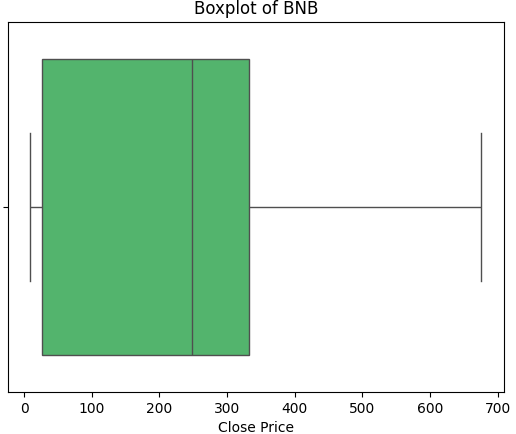
\includegraphics[width=1\textwidth]{image/bnb1.png}
    \caption{BNB price's boxplot}
    \label{fig:1}
    \end{minipage}
    \hfill
    \begin{minipage}{0.23\textwidth}
    \centering
    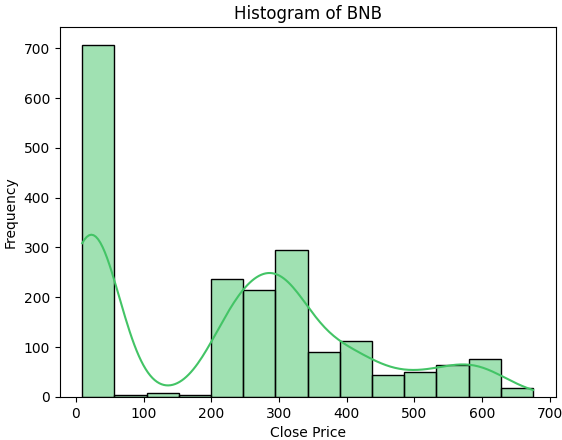
\includegraphics[width=1\textwidth]{image/bnb2.png}
    \caption{BNB price's histogram}
    \label{fig:2}
    \end{minipage}
\end{figure}

\begin{figure}[H]
    \centering
    \begin{minipage}{0.23\textwidth}
    \centering
    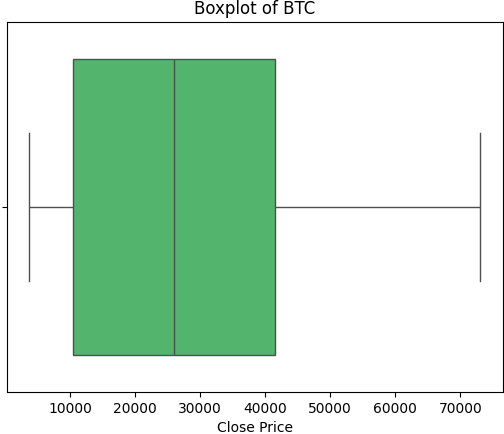
\includegraphics[width=1\textwidth]{image/btc1.png}
    \caption{BTC price's boxplot}
    \label{fig:1}
    \end{minipage}
    \hfill
    \begin{minipage}{0.23\textwidth}
    \centering
    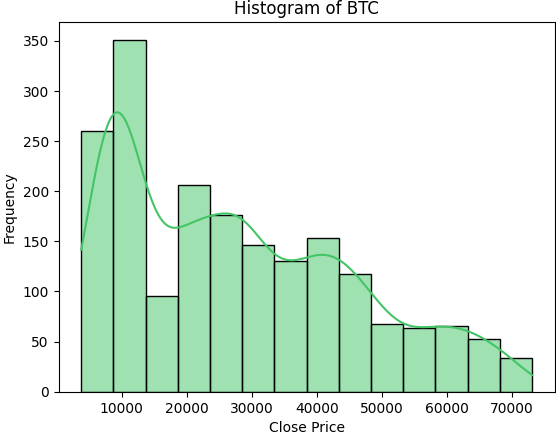
\includegraphics[width=1\textwidth]{image/btc2.png}
    \caption{BTC price's histogram}
    \label{fig:2}
    \end{minipage}
\end{figure}

\begin{figure}[H]
    \centering
    \begin{minipage}{0.23\textwidth}
    \centering
    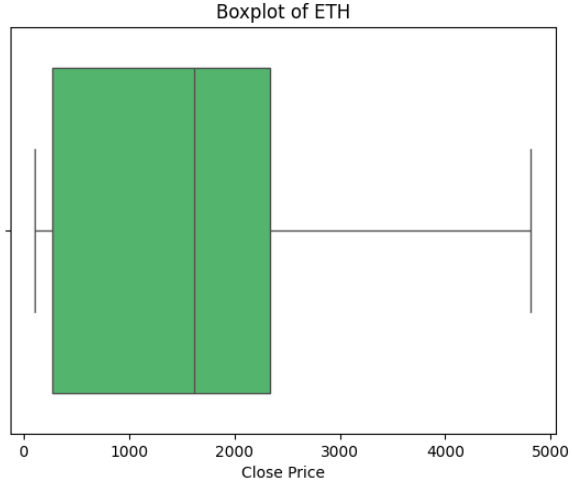
\includegraphics[width=1\textwidth]{image/eth1.png}
    \caption{ETH price's boxplot}
    \label{fig:1}
    \end{minipage}
    \hfill
    \begin{minipage}{0.23\textwidth}
    \centering
    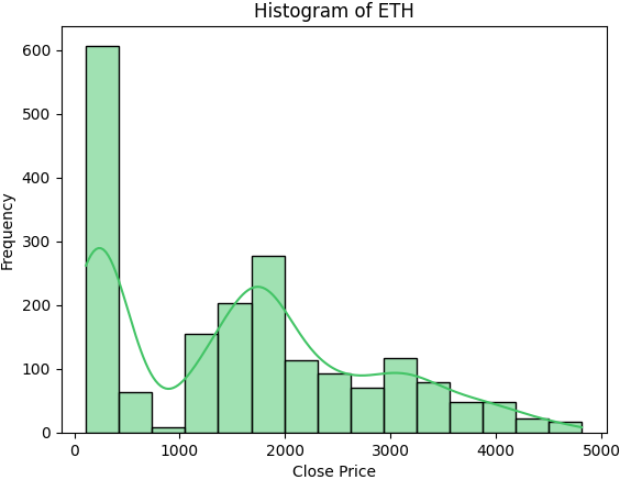
\includegraphics[width=1\textwidth]{image/eth2.png}
    \caption{ETH price's histogram}
    \label{fig:2}
    \end{minipage}
\end{figure}


\section{METHODOLOGY}
\subsection{Deployment}
\begin{figure}[H]
  \centering
  \begin{minipage}{0.9\linewidth}
    \centering
    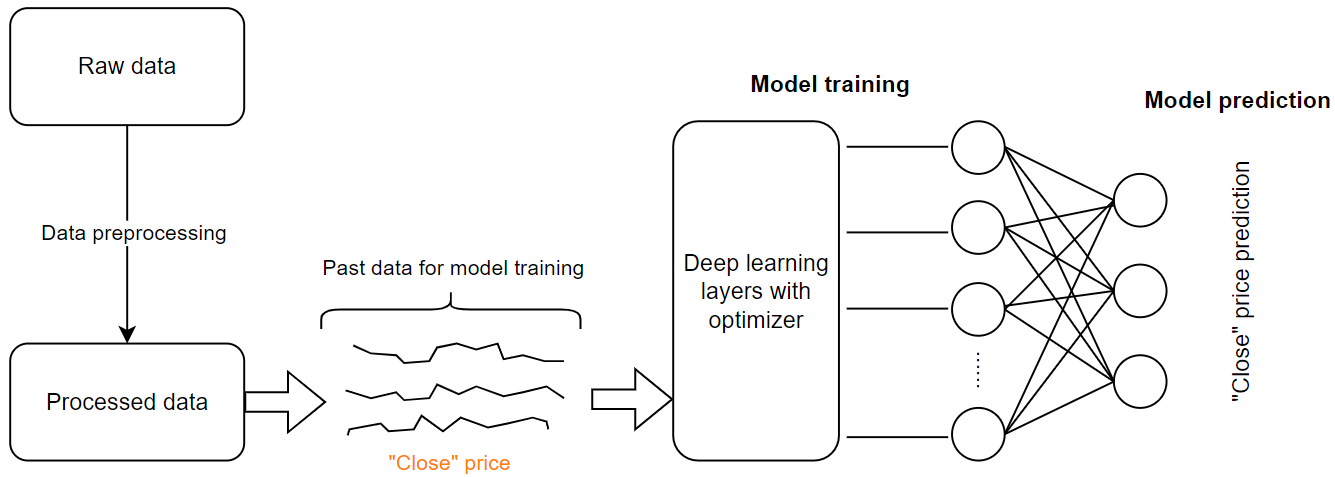
\includegraphics[width=\linewidth]{image/Deployment.png}
    \caption{The experimental procedure.}
    \label{fig8}
  \end{minipage}
\end{figure}
\textbf{Input:} Historical data on Cryptocurrency Prices consists of a lot of features: "Open", "High", "Low", "Close", "Adj Close", "Volume" on a daily basis from 1/3/2019 to 1/6/2024 for three datasets (BNB, BTC, ETH).\\
\textbf{Processing steps:} 
    \begin{itemize}
        \item Preprocessing the raw datasets.
        \item Then, using historical “Close” prices as the input values for model training.
        \item Finally, build regression models integrating with optimizers to minimize loss function.
    \end{itemize}
\textbf{Output:} “Close” prices prediction for three datasets (BNB, BTC, ETH).

\subsection{Models}
\subsubsection{LINEAR REGRESSION}
Linear regression is a statistical technique that involves creating a linear equation to represent the connection between a dependent variable and one or more independent variables, based on observed data. The main objective of linear regression is to determine a linear correlation between the independent variable(s) and the dependent variable, allowing for predictions or explanations of the dependent variable based on the values of the independent variable(s). The linear regression model is represented by the equation:
\[Y = \beta_0 + \beta_1 X_1 + \beta_2 X_2 + \ldots + \beta_n X_n + \epsilon\]
Where:\\
        \indent\textbullet\ \(Y\) is the dependent variable.\\
        \indent\textbullet\ \(X_1, X_2,...,X_n\) are the independent variables.\\
        \indent\textbullet\ \(\beta_0\) is the intercept (the value of Y when all independent variables are zero).\\
        \indent\textbullet\ \(\beta_1, \beta_2,..., \beta_n\) are the coefficients (representing the change in Y for a one-unit change in the corresponding X).\\
        \indent\textbullet\ \(\epsilon\) is the error term.
\subsubsection{ARIMA}
ARIMA, which stands for Autoregressive Integrated Moving Average, is a prevalent model employed for forecasting time series data. The model represents a multiple linear regression equation of input variables with the main components being:\\
Auto regression (AR): This model represents the relationship between the current data and p previous data points (lag). 
\[AR(p) = \alpha + \beta_1 y_{t-1} + \beta_2 y_{t-2} + \dots + \beta_p y_{t-p} + \varepsilon_t\]
Intergrated (I):This process involves cointegration or differencing.
\[I(1) = y_t - y_{t-1}\]
Moving average (MA): This model represents the relationship between the current data and previous errors. It involves shifting or changing the average value of the series over time.
\[MA(q) = \alpha + \theta_1 \varepsilon_{t-1} + \theta_2 \varepsilon_{t-2} + \dots + \theta_q \varepsilon_{t-q} + \varepsilon_t\]
So the equation of an ARIMA(p, d, q)model becomes :
\[y_t = \alpha + \beta_1 y_{t-1} + \beta_2 y_{t-2} + \dots + \beta_p y_{t-p} + \varepsilon_t + \]
\[\theta_1 \varepsilon_{t-1} + \theta_2 \varepsilon_{t-2} + \dots + \theta_q \varepsilon_{t-q}\]
Where:\\
	\indent\textbullet\ \(y_t\) is the forecast point at time t.\\
        \indent\textbullet\ \(\beta_p\) is the coefficient of each parameter p.\\
	\indent\textbullet\ \(\theta_p\) is the coefficient of each parameter q.\\
	\indent\textbullet\ \(\alpha\) is the intercept term or constant.\\
	\indent\textbullet\ \(\varepsilon_t\) is the white noise error term at time t.
\subsubsection{D-LINEAR}
"DLinear\cite{model_Dlinear}" stands for Decomposed Linear, a forecasting model that incorporates a decomposition approach similar to methods seen in Autoformer and FEDformer, combined with linear layers.  The key innovation of D-Linear is the decomposition of the input time series into trend and seasonal components, which are then modeled separately using simple linear layers before combining the results. This approach explicitly addresses the presence of trends in data, thereby enhancing the predictive performance compared to conventional linear models \cite{model_Dlinear}.
\begin{figure}[H]
  \centering
  \begin{minipage}{0.9\linewidth}
    \centering
    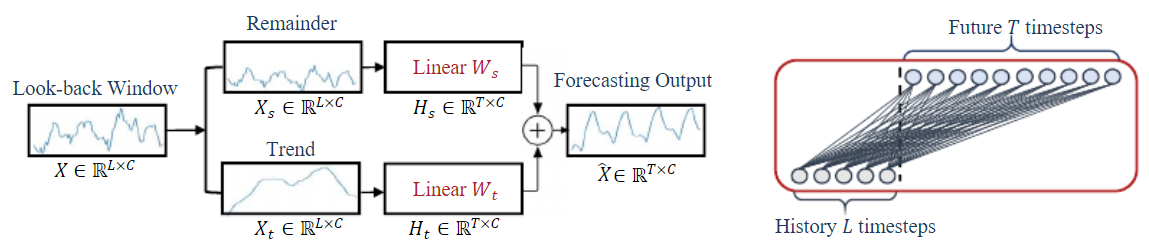
\includegraphics[width=\linewidth]{image/D-linear_1.png}
    \caption{Illustration of the of D-Linear\cite{model_Dlinear}.}
    \label{fig8}
  \end{minipage}
\end{figure}
\noindent "DLinear" initially decomposes a time-series dataset into its trend component \(X_{t} \in \mathbb{R}^{L \times C}\)\cite{model_Dlinear} and a residual component\(X_{s} = X-X_t\)\cite{model_Dlinear}. After this separation, each component is processed using distinct one-layer linear networks. The procedure can be summarized as follows: \(\hat {X} = H_s-H_t\)\cite{model_Dlinear}, where \(H_{s} = W_s X_s \in \mathbb{R}^{T \times C}\)\cite{model_Dlinear}  and  \(H_{t} = W_t X_t \in \mathbb{R}^{T \times C}\)\cite{model_Dlinear}  represent the decomposed remainder and trend features, respectively. Here, \(W_{s} \in \mathbb{R}^{T \times L}\)and \(W_{t} \in \mathbb{R}^{T \times L}\)\cite{model_Dlinear} denote two linear layers.
\subsubsection{RNN}
Recurrent Neural Networks (RNN) are a specific sort of neural network that is specifically built to handle and analyze input that is presented in a consecutive manner. RNNs, in contrast to conventional feedforward neural networks, has the capability to retain information from earlier stages by means of hidden states. This enables them to acquire knowledge of long-term relationships in sequential data, such as time series and natural language.
\begin{figure}[H]
  \centering
  \begin{minipage}{1\linewidth}
    \centering
    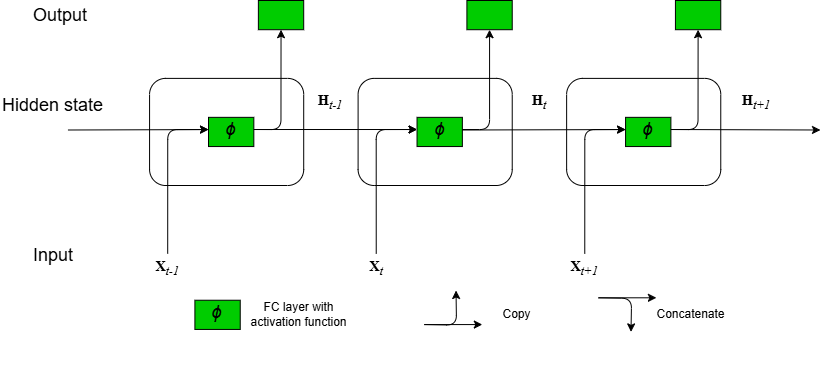
\includegraphics[width=\linewidth]{image/RNN1.png}
    \caption{RNN architecture.}
    \label{fig8}
  \end{minipage}
\end{figure}
\noindent State of Hidden Layer at Time-Step t.
\[H_t = \phi(X_t W_{xh} + H_{t-1} W_{hh} + b_h)\]
Output at Time-step t.
\[ O_t = H_t W_{hq} + b_q \]
Where:\\
	\indent\textbullet\ \(X_t\in \mathbb{R}^{n \times d}\) is input at time step \(t\).\\
        \indent\textbullet\ \(H_t\in \mathbb{R}^{n \times h}\) hidden state at time step \(t\).\\
	\indent\textbullet\ \(W_{xh}\in \mathbb{R}^{d \times h}\) hidden state weight matrix at time-step \(t\).\\
	\indent\textbullet\ \(b_h\in \mathbb{R}^{1 \times h}\) hidden state bias coefficient at time-step \(t\).\\
	\indent\textbullet\ \(H_{t-1}\) hidden state at time-step \(t-1\).\\
        \indent\textbullet\  \(W_{hh} \in \mathbb{R}^{h \times h}\) hidden state weight matrix at time-step \(t-1\).\\
        \indent\textbullet\ \(W_{hq} \in \mathbb{R}^{h \times q}\) output layer weight matrix at time-step \(t\).\\
        \indent\textbullet\ \(b_q \in \mathbb{R}^{1 \times h}\) output layer bias coefficient at time-step \(t\).\\
        \indent\textbullet\ \(\phi\) activation function (it could be tanh or sigmoid).      

\subsubsection{LSTM}
An enhancement of RNNs intended to address their drawbacks in long-term dependency learning is Long short-term memory. Long-term dependencies refer to the influence of input values from the beginning to the output values. LSTM has the ability to remember and maintain information over a long period of time, which is challenging for traditional RNNs. For short-term memory, an LSTM has a hidden state, and for long-term memory, it has a cell state. 
\begin{figure}[H]
  \centering
  \begin{minipage}{1\linewidth}
    \centering
    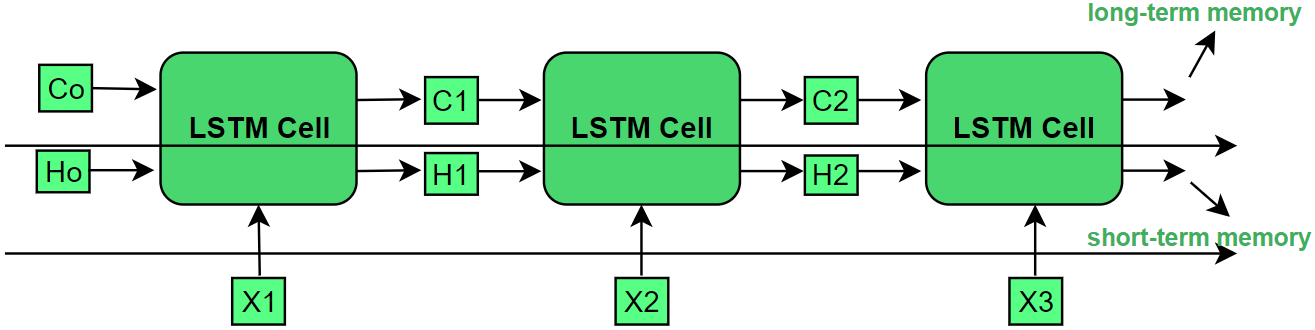
\includegraphics[width=\linewidth]{image/LSTM1.png}
    \caption{Overview of LSTM.}
    \label{fig8}
  \end{minipage}
\end{figure}
\noindent An input gate, a forget gate, and an output gate are the three primary parts of an LSTM unit.
\begin{figure}[H]
  \centering
  \begin{minipage}{0.8\linewidth}
    \centering
    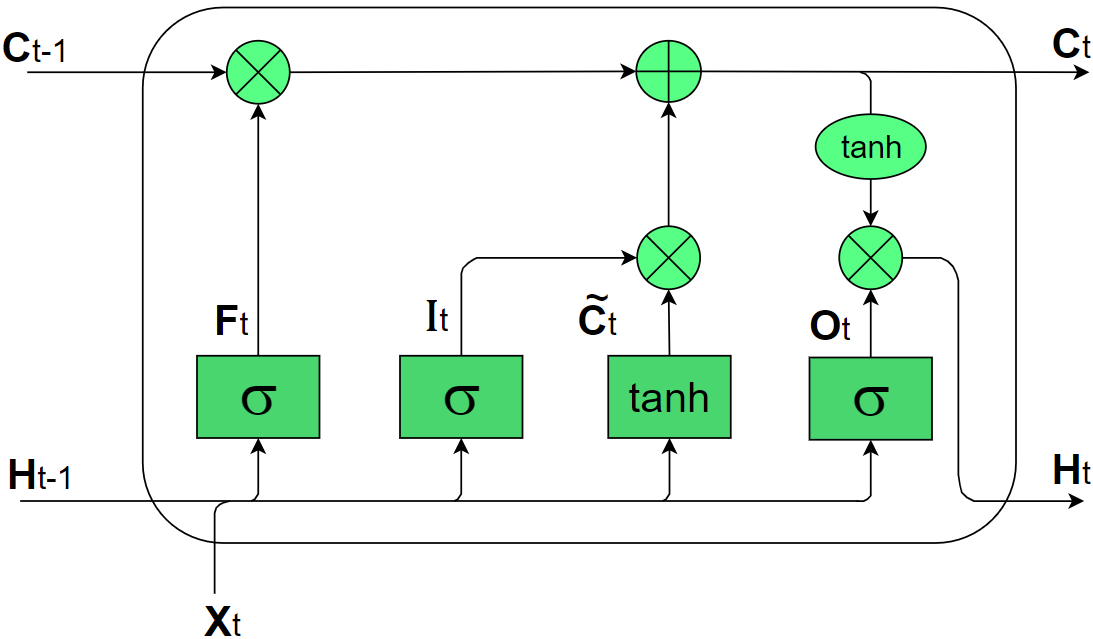
\includegraphics[width=\linewidth]{image/LSTM2.png}
    \label{fig8}
  \end{minipage}
  \caption{ LSTM architecture.}
\end{figure}
\noindent
\textbf{Forget Gate:} This gate determines which information should be retained or discarded.
\[F_t = \sigma(X_tW_{xf} + H_{t-1}W_{hf}+ b_f)\]
\textbf{Input Gate:} it decides the amount of new information should be added to the cell state \(C_t\) from the current input \(X_t\) and the previous hidden state \(h_{t-1}\) .
\[I_t = \sigma(X_tW_{xi} + H_{t-1}W_{hi}+ b_i)\]
\textbf{Candidate Cell State:} This vector represents potential new information to be added to the cell state.
\[\widetilde{C}_t = \tanh\ (X_t W_{xc} + H_{t-1} W_{hc} + b_c)\]
\textbf{Cell State:}\[C_t = (F_t\cdot C_{t-1}) + I_{t}\cdot\widetilde{C}_t\]
\textbf{Output Gate:} The output gate determines the value of the subsequent hidden state.	
\[O_t = \sigma(X_tW_{xo} + H_{t-1}W_{ho}+ b_o)\]
\textbf{Hidden state}:\[H_t = O_t\cdot tanh({C}_t)\]
Where:\\
	\indent\textbullet\ \(X_t\): the input at time t.\\
        \indent\textbullet\ \(H_{t-1}\) is the layer's previously hidden state.\\
        \indent\textbullet\ \(H_t\) is the hidden state at time t.\\
	\indent\textbullet\ \(W_{xf}, W_{hf}, W_{xi},W_{hi}, W_{xc}, W_{hc}, W_{xo}, W_{ho}\) are weight matrices.\\
	\indent\textbullet\ \(b_f, b_i, b_o\) are bias vectors.\\
	\indent\textbullet\ \(\sigma\): sigmoid activation function.\\
        \indent\textbullet\ tanh: tanh activation function.\\

\subsubsection{GRU}
GRUs, released by \cite{model_Gru}, offer a simpler alternative to LSTM units to address their complexity. GRUs have fewer trainable parameters because they lack the output layers presented in LSTMs. Figure below shows a single GRU unit.

\begin{figure}[H]
  \centering
  \begin{minipage}{0.8\linewidth}
    \centering
    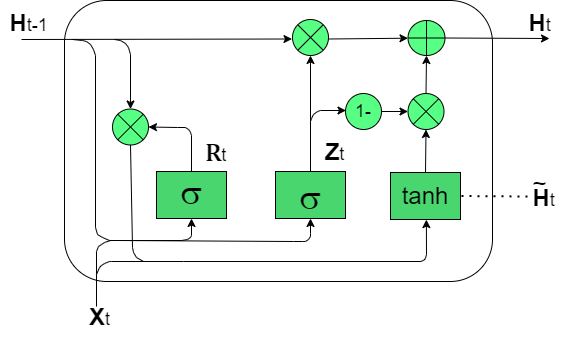
\includegraphics[width=\linewidth]{image/GRU.png}
    \label{fig8}
  \end{minipage}
  \caption{GRU architecture.}
\end{figure}
\noindent
LSTMs have three gates (input, output, and forget), but GRUs only have two (reset and update). \\
\textbf{Reset gate}: manages how new inputs are blended with stored information: \[R_t = \sigma(X_tW_{xr} + H_{t-1}W_{hr}+ b_r)\]\\
\textbf{Update gate}: controls how much of the previous state is preserved. The update gate in GRU model effectively serves as the input and forget gates combined in an LSTM.
\[Z_t = \sigma(X_tW_{xz} + H_{t-1}W_{hz}+ b_z)\]
GRUs do not have a distinct cell state like LSTMs do \(C_t\) in each unit. 
Thus, while GRUs are quite similar to LSTMs, their reduced complexity and fewer parameters make them an intriguing architecture for performance comparison with LSTMs in various scenarios, such as pouring.\\
\textbf{Candidate Hidden State}: represents the new information to be added to the hidden state.
\[\widetilde{H}_t = \tanh \left( X_t W_{xh} + (R_t \cdot H_{t-1}) W_{hh} + b_h \right)\]
\textbf{Hidden state}:\[H_t = (Z_t \cdot H_{t-1}) + (1-Z_t)\cdot \widetilde{H}_t \]
\textbf{Where:}\\
	\indent\textbullet\ \(X_t\): the input at time t.\\
        \indent\textbullet\ \(H_{t-1}\) is the layer’s previously hidden state.\\
	\indent\textbullet\ \(W_{xr}, W_{hr}, W_{xz}, W_{hz}, W_{xh}, W_{hh}\) are weight matrices.\\
	\indent\textbullet\ \(b_r, b_z, b_h\) are bias vectors.\\
	\indent\textbullet\ \(\sigma\) sigmoid activation function.\\
        \indent\textbullet\ tanh activation function.\\
\subsection{Optimizer}
Optimizers are crucial algorithms in deep learning since they dynamically modify a model's parameters as it is being trained in order to decrease a certain loss function. These techniques improve neural network learning by iteratively adjusting the biases and weights according to feedback from the data. Stochastic Gradient Descent (SGD), Adam, Adamax, Momentum, RMSprop, and Ftrl are well-liked deep learning optimizers. To increase overall performance, each optimizer has different momentum algorithms, learning rates, and update rules that all work together to find and converge on the ideal model parameters. \cite{opti}.
\subsubsection{ADAM}
Adam is a first-order gradient-based optimization method based on adaptive estimations of lower-order moments that is intended for stochastic objective functions. Adam modifies network weights iteratively using the training data, in contrast to the conventional Stochastic Gradient Descent (SGD) method \cite{Adam_1}. It makes intuitive sense to combine the "gradient descent with momentum" and "RMSP" algorithms.\cite{Adam_2}.
According to \cite{Adam_3} Adam can be likened to the Heavy Ball with Friction (HBF) (see below) method due to its averaging of past gradients, which corresponds to a velocity that helps prevent the optimizer from being trapped in small regions. This property allows Adam to typically overshoot small local minima, which can lead to mode collapse, and instead find flatter minima that generalize better.
\begin{figure}[H]
  \centering
  \begin{minipage}{0.7\linewidth}
    \centering
    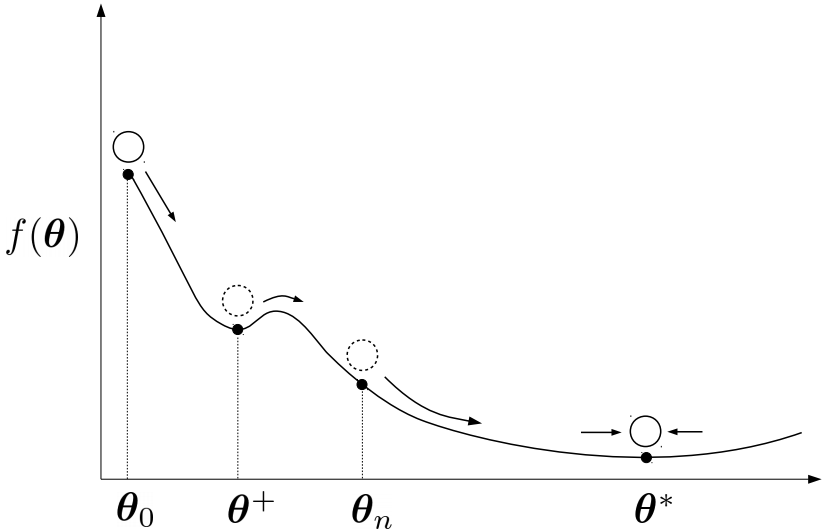
\includegraphics[width=\linewidth]{image/Adam1.png}
    \label{fig8}
  \end{minipage}
\caption{Heavy Ball with Friction, this scenario occurs when a mass ball surpasses the local minimum $\theta\sp{+}$ and ultimately reaches the flat minimum. $\theta\sp{*}$ }.
\end{figure}
\noindent We recapitulate the Adam update rule at step t:\\
\textbf{Get gradients w.r.t. stochastic objective at time step t\cite{Adam_4}:} 
\[\ g_t \leftarrow \nabla_\theta f_t (\theta_{t-1})\]
\textbf{Update biased first moment estimate\cite{Adam_4}: } 
\[\ m_t \leftarrow \beta_1 \cdot m_{t-1} + (1 - \beta_1) \cdot g_t\]
\textbf{Update biased second raw moment estimate: } 
\[\ v_t \leftarrow \beta_2 \cdot v_{t-1} + (1 - \beta_2) \cdot {g_t}\sp{2}\]
\textbf{Compute bias-corrected first moment estimate\cite{Adam_4}: } 
\[\ \hat{m_t} \leftarrow \frac{m_t}{1 - {\beta_1}\sp{t}}\]
\textbf{Compute bias-corrected second raw moment estimate\cite{Adam_4}: } 
\[\ \hat{v_t} \leftarrow \frac{v_t}{1 - {\beta_2}\sp{t}}\]
\textbf{Update parameters\cite{Adam_4}: } 
\[\ \theta_t \leftarrow  \theta_{t-1} - \alpha \cdot \frac {\hat{m_t}} {\sqrt{\hat{v_t}} + \epsilon}\]
Where: \\
        \indent\textbullet\ ${g_t}^2$ indicates the element-wise square ${g_t} \odot {g_t}$.\\
        \indent\textbullet\ $\alpha$ learning rate ($\alpha$ = 0.001).\\
        \indent\textbullet\ $\beta_1, \beta_2 \in [0, 1)$: exponential decay rates for the moment estimates. ($\beta_1 = 0.9$, $\beta_2 = 0.999$).\\
        \indent\textbullet\ $f_(\theta)$ stochastic objective function with parameters $\theta$. \\
        \indent\textbullet\ $\theta_0$ initial parameter vector.\\
        \indent\textbullet\ $m_0$ = 0 (Initialize 1st moment vector).\\
        \indent\textbullet\ $v_0$ = 0 (Initialize 2nd moment vector).\\
        \indent\textbullet\ $t$ = 0 (Initialize timestep).\\
        \indent\textbullet\ $\epsilon$: A small positive constant ($10^{-8}$) to avoid 'division by 0' error when ($v_t$ $\rightarrow$ 0).\\
        \indent\textbullet\ \({\beta_1}\sp{t}, {\beta_2}\sp{t}\) : $\beta_1$ and $\beta_2$ to the power t.\\
\subsubsection{ADAMAX}
Adamax is an optimization algorithm derived from Adam (Adaptive Moment Estimation), proposed by Kingma and Ba in "Adam: A Method for Stochastic Optimization" (2014). It extends Adam by using the infinity norm (maximum norm) instead of the L2 norm, offering better performance in some cases\cite{Adamax_1}.\\
Adamax combines the strengths of AdaGrad and RMSProp while addressing their limitations. It adapts the learning rates for each parameter based on the first and second moments of the gradients. Using the infinity norm, Adamax maintains robust parameter updates even with sparse gradients.
Initialization: Initialize the parameters $\theta_0$, the first moment vector $\mathbf{m}_0$, and the exponentially weighted infinity norm $\mathbf{u}_0$: $\ m_0 = 0$, $\ u_0 = 0$\\
Update Rule at each time step t:\\
\textbf{Compute the gradient of the objective function with respect to} $\ g_{t} = \nabla_{\theta} J \theta_{t-1}$\\
\textbf{Update biased first moment estimate}
\[\ m_{t} = \beta_{1} m_{t-1}  + (1-\beta_1) g_t\] 
\textbf{Update exponentially weighted infinity norm}
\[\ u_t = max(\beta_{2} u_{t-1}, \vert{g_t}\vert) \]
\textbf{Compute bias-corrected first moment estimate}
\[\ \hat{m_t} = \frac{m_t}{1 - {\beta_1}\sp{t}}\] 
\[\ \theta_{t} = \theta_{t-1} - \eta\frac{\hat {m^t}}{u_t}\] 
Where: \\
        \indent\textbullet\ $\beta_1, \beta_2$ are hyperparameters for controlling the exponential decay rates for the moment estimates, typically set to $\beta_1 = 0.9 $ and $\beta_2 = 0.999..$\\
        \indent\textbullet\ $\eta$ is the learning rate.\\
        \indent\textbullet\ $\nabla_{\theta} J \theta_{t-1}$: denotes the gradient of the objective function J with respect to the parameters $\theta$.
        
\subsubsection{FTRL}
The Follow-the-Regularized-Leader (FTRL) optimizer is an advanced optimization algorithm used extensively in machine learning, particularly for tasks involving large-scale and sparse datasets. It is particularly effective for online learning scenarios, making it a valuable tool for forecasting applications such as predicting cryptocurrency prices. This section elaborates on the theoretical underpinnings of the FTRL optimizer, detailing its algorithm and its suitability for time series deep learning models \cite{Ftrl_1}.\\
\textbf{Theoretical Foundations:} 
The FTRL optimizer originates from the framework of online convex optimization, where the objective is to iteratively minimize a convex loss function. In each iteration t,the learner aims to select a weight vector $\ w_t$ that minimizes the cumulative loss, given by
\[\displaystyle \sum_{i=1}^{t} l_i(w) \]
Where$\ l_i(w)$ is the loss at iteration$\ i$. FTRL optimizes this by incorporating a regularization term, which helps in controlling the complexity of the model and preventing overfitting.\\
\textbf{Algorithmic Formulation:} The core idea of FTRL is to follow the regularized leader, i.e., to select weights that minimize the regularized cumulative loss. The update rule for FTRL can be described as follows:
\begin{itemize}
    \item \textbf{Initialize:} Start with initial weights w1 , typically set to zero
    \item \textbf{Gradient Accumulation:} Maintain a cumulative gradient vector gt , which is sum of gradients of the loss functions up to the current iteration:
    \[\ g_t = \displaystyle \sum_{i=1}^{t} \nabla l_i(w) \]
    \item \textbf{Weight Update:} At each iteration t, update the weights according to:
    \[\ w_{t+1} = argmin_w \left( g_t \cdot w + \frac{1}{2\eta_t} \|w\|^2 + R(w) \right)\]
\end{itemize}

\textbf{Where:} \\
        \indent\textbullet\ \( g_t \cdot w\) represents the inner product of the cumulative gradient and the weight vector.\\
        \indent\textbullet\ \(\eta_t\) is the learning rate at iteration t.\\
        \indent\textbullet\ \(\| w \|\) is the regularization term.\\
        \indent\textbullet\ \(R(w)\) is an additional regularization term that can be used to incorporate different forms of regularization, such as L1 regularization for promoting sparsity.\\

\section{RESULTS}
\subsection{METRICS}
\par In this study, the performance of the forecasting models was evaluated using two primary assessment measures:\\
\textbf{Mean Absolute Percentage Error (MAPE):} The average percentage difference between the actual and predicted values for a certain time period n is determined by this metric. Through the display of the rate difference between the predicted and actual numbers, it offers a relative gauge of the model's accuracy. Equation is used to express it:
\[\ MAPE = \frac{1}{n}\sum_{t=1}^{n} \left|\frac{y_t - \hat{y}_t}{y_t}\right| \cdot {100} \]
\textbf{Mean Absolute Error (MAE):} The average absolute difference between the actual and predicted values for a specified time period is determined by this metric. It gives an exact assessment of the accuracy of the model and is expressed by the following equation:
\[\ MAE = \frac{1}{n}\sum_{t=1}^{n} \left|{y_t - \hat{y}_t}\right|\]
Additionally, \textbf{Root Mean Squared Error (RMSE)} was employed as the models' training loss function. The square root of the average of the squared discrepancies between the observed and predicted values over a certain time period is evaluated using RMSE using the following n equation:
\[\ RMSE = \sqrt{\frac{1}{n}\sum_{t=1}^{n} (y_t - \hat{y}_t)^2}\] 

\subsection{RESULTS}
The performance of many models, including deep learning models DLinear, RNN, LSTM, and GRU, each combined with Adam Optimizer, Adamax Optimizer, and Ftrl Optimizer, is shown in the comparison findings in the three tables below. Besides, we also implement Machine learning models namely Linear Regression (LR) and ARIMA.\\
\subsubsection{BNB DATASET}
\definecolor{ao(english)}{rgb}{0.263, 0.769, 0.400}
\begin{table}[H]
    \centering
    \caption{Performance Metrics for Various Models and Optimizers}
    \begin{tabular}{|c|c|c|c|c|c|}
        \hline
        \rowcolor{ao(english)}
        Model & Proportion & Optimizer & RMSE & MAPE (\%) & MAE \\ \hline
        
        \multirow{6}{*}{D-Linear} & \multirow{3}{*}{7:3} & Adam & 161.36 & 33.81 & 112.19 \\ \cline{3-6}
         &  & Adamax & 157.80 & 33.13 & 109.34 \\ \cline{3-6}
         &  & \textbf{Ftrl} & \textbf{142.59} & \textbf{26.09} & \textbf{97.85} \\ \cline{2-6}
         & \multirow{3}{*}{8:2} & Adam & 193.80 & 40.65 & 139.64 \\ \cline{3-6}
         &  & Adamax & 190.65 & 42.30 & 138.58 \\ \cline{3-6}
         &  & \textbf{Ftrl} & \textbf{169.53} & \textbf{30.87} & \textbf{119.46} \\ \cline{2-6}
         & \multirow{3}{*}{9:1} & Adam & 199.93 & 41.22 & 158.36 \\ \cline{3-6}
         &  & Adamax & 200.50 & 40.30 & 159.05 \\ \cline{3-6}
         &  & Ftrl & 207.61 & 33.66 & 168.82 \\ \hline

        \multirow{9}{*}{RNN} & \multirow{3}{*}{7:3} & Adam & 77.18 & 2.52 & 52.24 \\ \cline{3-6}
         &  & \textbf{Adamax} & \textbf{15.21} & \textbf{3.58} & \textbf{11.38} \\ \cline{3-6}
         &  & Ftrl & 197.45 & 44.58 & 159.76 \\ \cline{2-6}
         & \multirow{3}{*}{8:2} & \textbf{Adam} & \textbf{14.93} & \textbf{2.51} & \textbf{9.37} \\ \cline{3-6}
         &  & Adamax & 19.12 & 4.61 & 14.93 \\ \cline{3-6}
         &  & Ftrl & 209.15 & 39.02 & 155.82 \\ \cline{2-6}
         & \multirow{3}{*}{9:1} & \textbf{Adam} & \textbf{19.02} & \textbf{2.8} & \textbf{13.07} \\ \cline{3-6}
         &  & Adamax & 26.5 & 6.38 & 22.29 \\ \cline{3-6}
         &  & Ftrl & 260.16 & 44.5 & 217.17 \\ \hline

        \multirow{9}{*}{LSTM} & \multirow{3}{*}{7:3} & \textbf{Adam} & \textbf{12.44} & \textbf{2.96} & \textbf{9.19} \\ \cline{3-6}
         &  & Adamax & 17.96 & 4.19 & 13.27 \\ \cline{3-6}
         &  & Ftrl & 166.26 & 30.69 & 119.06 \\ \cline{2-6}
         & \multirow{3}{*}{8:2} & \textbf{Adam} & \textbf{11.94} & \textbf{2.21} & \textbf{7.51} \\ \cline{3-6}
         &  & Adamax & 16.72 & 4.02 & 12.63 \\ \cline{3-6}
         &  & Ftrl & 182.20 & 26.22 & 118.21 \\ \cline{2-6}
         & \multirow{3}{*}{9:1} & \textbf{Adam} & \textbf{17.21} & \textbf{2.57} & \textbf{11.54} \\ \cline{3-6}
         &  & Adamax & 30.00 & 4.83 & 22.94 \\ \cline{3-6}
         &  & Ftrl & 252.64 & 42.03 & 207.91 \\ \hline
         
        \multirow{9}{*}{GRU} & \multirow{3}{*}{7:3} & \textbf{Adam} & \textbf{14.44} & \textbf{3.73} & \textbf{11.57} \\ \cline{3-6}
         &  & Adamax & 19.44 & 5.77 & 17.10 \\ \cline{3-6}
         &  & Ftrl & 279.60 & 76.88 & 254.38 \\ \cline{2-6}
         & \multirow{3}{*}{8:2} & \textbf{Adam} & \textbf{13.25} & \textbf{2.64} & \textbf{8.90} \\ \cline{3-6}
         &  & Adamax & 13.78 & 2.21 & 8.37 \\ \cline{3-6}
         &  & Ftrl & 292.68 & 73.92 & 257.29 \\ \cline{2-6}
         & \multirow{3}{*}{9:1} & \textbf{Adam} & \textbf{15.04} & \textbf{2.20} & \textbf{9.57} \\ \cline{3-6}
         &  & Adamax & 15.64 & 2.52 & 10.49 \\ \cline{3-6}
         &  & Ftrl & 367.69 & 76.65 & 338.52 \\ \hline
         
        \multirow{3}{*}{LR} & 7:3 &  & 250.68 & 86.55 & 231.04 \\ \cline{2-6}
         & 8:2 &  & 196.76 & 69.90 & 178.59 \\ \cline{2-6}
         & 9:1 &  & \textbf{131.97} & \textbf{32.99} & \textbf{124.80}
 \\ \hline

        \multirow{3}{*}{ARIMA} & 7:3 &  & \textbf{116.06} & \textbf{24.38} & \textbf{81.92}
 \\ \cline{2-6}
         & 8:2 &  & 141.27 & 30.02 & 106.91 \\ \cline{2-6}
         & 9:1 &  & 244.68 & 39.45 & 198.19 \\ \hline


    \end{tabular}
\end{table}
\textbf{Prediction next 30/60/90 days (the best models)}





\begin{figure}[H]
  \centering
  \begin{minipage}{0.48\linewidth}
    \centering
    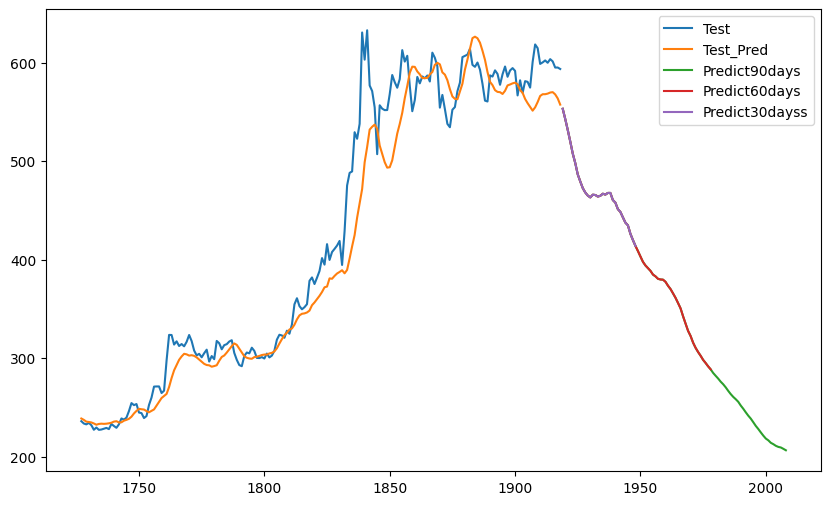
\includegraphics[width=1\textwidth]{image/BNB_DLinear_91_Adam.png}
    \caption{BNB DLinear 91 Adam}
    \label{fig:bnb-dlinear}
  \end{minipage}
  \hfill
  \begin{minipage}{0.48\linewidth}
    \centering
    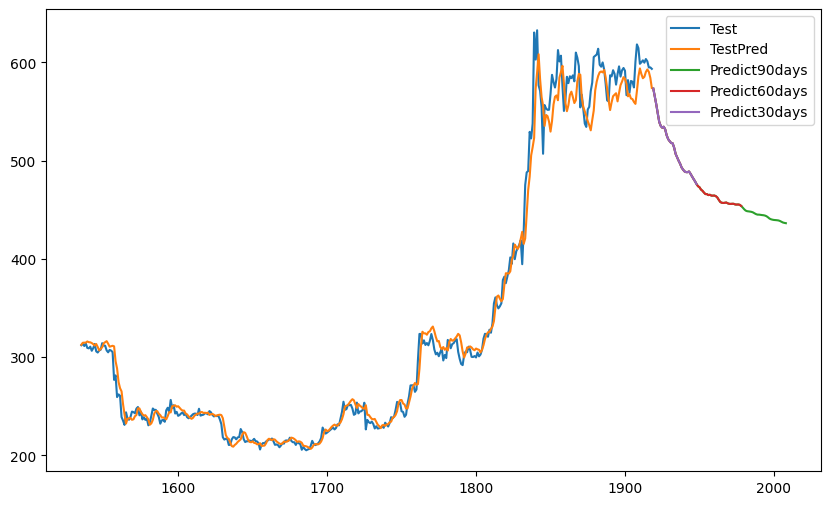
\includegraphics[width=1\textwidth]{image/BNB_RNN_82_Adam.png}
    \caption{BNB RNN 82 Adam}
    \label{fig:bnb-rnn}
  \end{minipage}
\end{figure}
% ////
\begin{figure}[H]
  \centering
  \begin{minipage}{0.48\linewidth}
    \centering
    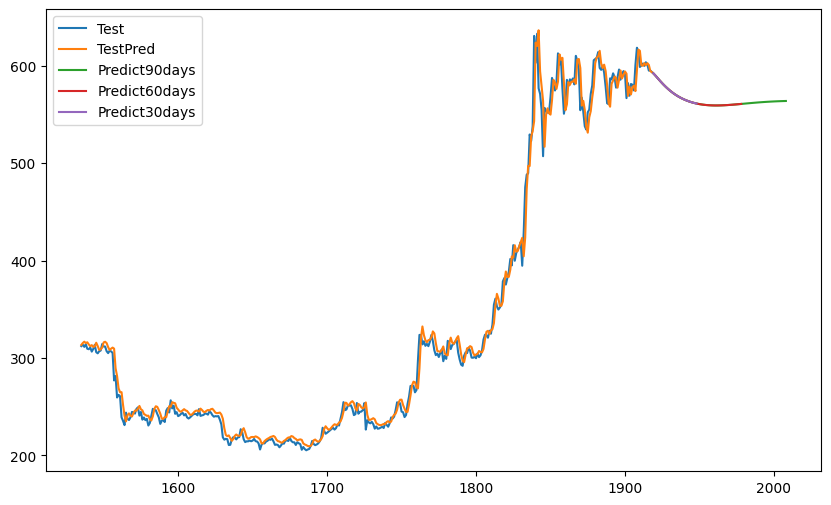
\includegraphics[width=1\textwidth]{image/BNB_LSTM_82_Adam.png}
    \caption{BNB LSTM 82 Adam.}
  \end{minipage}  
  \hfill
  \begin{minipage}{0.48\linewidth}
    \centering
    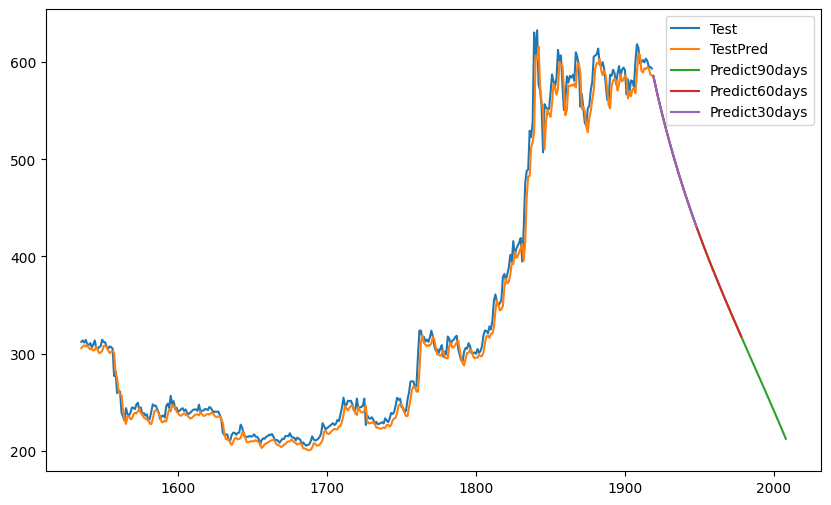
\includegraphics[width=1\textwidth]{image/BNB_GRU_82_Adam.png}
    \caption{BNB GRU 82 Adam.}
  \end{minipage}  
\end{figure}


\begin{figure}[H]
  \centering
  \begin{minipage}{0.48\linewidth}
    \centering
    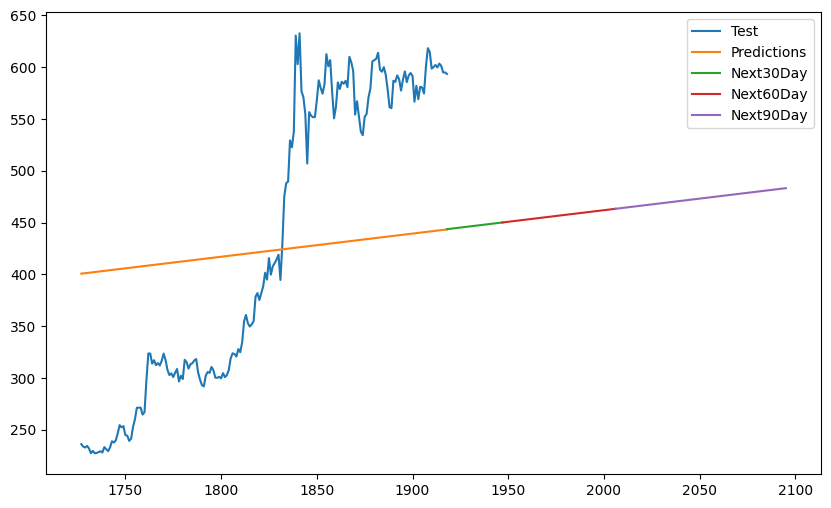
\includegraphics[width=1\linewidth]{image/BNB_LR_91.png}
    \caption{BNB LR 91.}
  \end{minipage}  
    \hfill
  \begin{minipage}{0.48\linewidth}
    \centering
    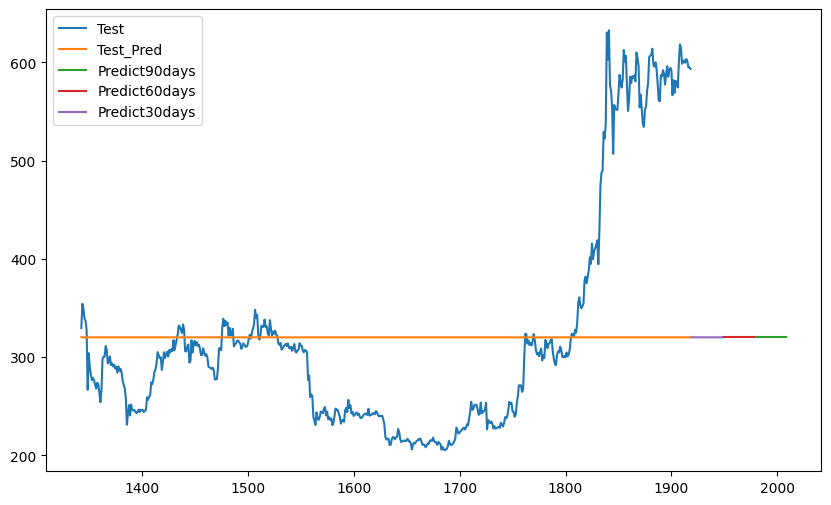
\includegraphics[width=1\linewidth]{image/BNB_ARIMA_73.png}
    \caption{BNB ARIMA 73.}
  \end{minipage}  
\end{figure}
% ///////////////////////////


\subsubsection{BTC DATASET}
\begin{table}[H]
    \centering
    \caption{Performance Metrics for Various Models and Optimizers}
    \definecolor{orange}{rgb}{1.0, 0.65, 0.0}
    \begin{tabular}{|c|c|c|c|c|c|}
        \hline
        \rowcolor{ao(english)}
        Model & Prop & Opti & RMSE & MAPE (\%) & MAE \\ \hline
        
        \multirow{6}{*}{D-Linear} & \multirow{3}{*}{7:3} & Adam & 21860.36 & 50.34 & 16513.02 \\ \cline{3-6}
         &  & Adamax & 21688.53 & 49.83 & 16359.17 \\ \cline{3-6}
         &  & \textbf{Ftrl} & \textbf{19608.7} & \textbf{39.74} & \textbf{14557.06} \\ \cline{2-6}
         & \multirow{3}{*}{8:2} & Adam & 21253.18 & 40.87 & 16514.89 \\ \cline{3-6}
         &  & Adamax & 21177.52 & 40.45 & 16393.89 \\ \cline{3-6}
         &  & \textbf{Ftrl} & \textbf{19736.55} & \textbf{32.36} & \textbf{14954.5} \\ \cline{2-6}
         & \multirow{3}{*}{9:1} & \textbf{Adam} & \textbf{16090.47} & \textbf{24.04} & \textbf{12847.67} \\ \cline{3-6}
         & & Adamax & 16202.79 & 24.12 & 12883.69\\ \cline{3-6}
         &  & Ftrl & 19546.67 & 27.41 & 16204.66 \\ \hline
         
        \multirow{9}{*}{RNN} & \multirow{3}{*}{7:3} & \textbf{Adam} & \textbf{1865.6} & \textbf{2.77} & \textbf{1141.21} \\ \cline{3-6}
         &  & Adamax & 1903.64 & 5.05& 1602.01 \\ \cline{3-6}
         &  & Ftrl & 27453.17 & 56.19 & 22385.58 \\ \cline{2-6}
         & \multirow{3}{*}{8:2} & \textbf{Adam} & \textbf{1663.14} & \textbf{2.25} & \textbf{1070.36} \\ \cline{3-6}
         &  & Adamax & 1801.49 & 2.6 & 1207.35 \\ \cline{3-6}
         &  & Ftrl & 22807.83 & 32.8 & 16953.98 \\ \cline{2-6}
         & \multirow{3}{*}{9:1} & \textbf{Adam} & \textbf{2185.82} & \textbf{2.94} & \textbf{1671.48} \\ \cline{3-6}
         &  & Adamax & 3372.15 & 4.48 & 2661.25 \\ \cline{3-6}
         &  & Ftrl & 32487.44 & 53.05 & 30296.7 \\ \hline
         
        \multirow{9}{*}{LSTM} & \multirow{3}{*}{7:3} & \textbf{Adam} & \textbf{1208.22} & \textbf{2.05} & \textbf{753.17} \\ \cline{3-6}
         &  & Adamax & 1800.43 & 3.24 & 1192.07 \\ \cline{3-6}
         &  & Ftrl & 18392.06 & 28.74 & 12258.09 \\ \cline{2-6}
         & \multirow{3}{*}{8:2} & \textbf{Adam} & \textbf{1462.8} & \textbf{2.78} & \textbf{1130.96} \\ \cline{3-6}
         &  & Adamax & 1682.23 & 2.87 & 1228.1 \\ \cline{3-6}
         &  & Ftrl & 22489.04 & 30.87 & 16306.55 \\ \cline{2-6}
         & \multirow{3}{*}{9:1}& Adam & 2377.73 & 3.21 & 1834.47 \\ \cline{3-6}
         & & \textbf{Adamax} & \textbf{1959.13} & \textbf{2.67} & \textbf{1485.52} \\
         \cline{3-6}
         &  & Ftrl & 31077.25 & 50.13 & 28772.75 \\ \hline

         \multirow{9}{*}{GRU} & \multirow{3}{*}{7:3} & \textbf{Adam} & \textbf{1217.21} & \textbf{1.88} & \textbf{732.36} \\ \cline{3-6}
         &  & Adamax & 1268.38 & 2.55 & 876.17 \\ \cline{3-6}
         &  & Ftrl & 29173.85 & 63.16 & 24465.3 \\ \cline{2-6}
         & \multirow{3}{*}{8:2} & \textbf{Adam} & \textbf{1339.02} & \textbf{2.3} & \textbf{961.87} \\ \cline{3-6}
         &  & Adamax & 1397.79 & 1.95 & 888.98 \\ \cline{3-6}
         &  & Ftrl & 35117.15 & 71.82 & 31514.48 \\ \cline{2-6}
         & \multirow{3}{*}{9:1} & Adam & 1903.98 & 2.33 & 1348.14 \\
        \cline{3-6}
         &  & \textbf{Adamax} & \textbf{1763.44} & \textbf{2.22} & \textbf{1250.56} \\ \cline{3-6}
         &  & Ftrl & 41903.72 & 72.02 & 40224.34 \\ \hline
         
        \multirow{3}{*}{LR} & 7:3 &  & 21165.54 & 74.94 & 19616.68 \\ \cline{2-6}
         & 8:2 &  & \textbf{13613.07} & \textbf{30.1} & \textbf{11676.31} \\ \cline{2-6}

         & 9:1 &  & 19042.08 & 25.2 & 15563.09 \\ \hline

        \multirow{3}{*}{ARIMA} & 7:3 &  & 22051.23 & 36.87 & 16038.92 \\ \cline{2-6}
         & 8:2 &  & \textbf{21700.03} & \textbf{28.55} & \textbf{15372.64} \\ \cline{2-6}

         & 9:1 &  & 22331.36 & 31.43 & 18993.83 \\ \hline
         
    \end{tabular}
\end{table}

\textbf{Prediction next 30/60/90 days (the best models)}
\begin{figure}[H]
  \centering
  \begin{minipage}{0.48\linewidth}
    \centering
    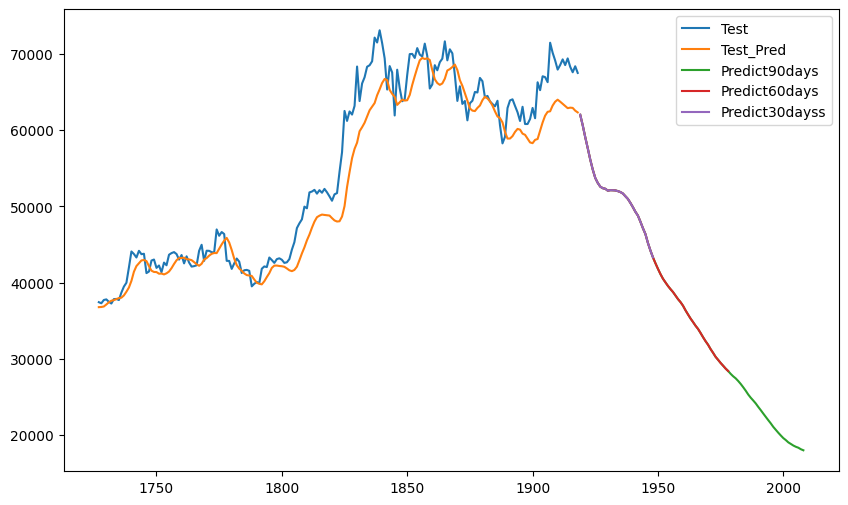
\includegraphics[width=1\linewidth]{image/BTC_DLinear_91_Adam.png}
    \caption{BTC DLinear 91 Adam.}
  \end{minipage}
  \hfill
  \begin{minipage}{0.48\linewidth}
    \centering
    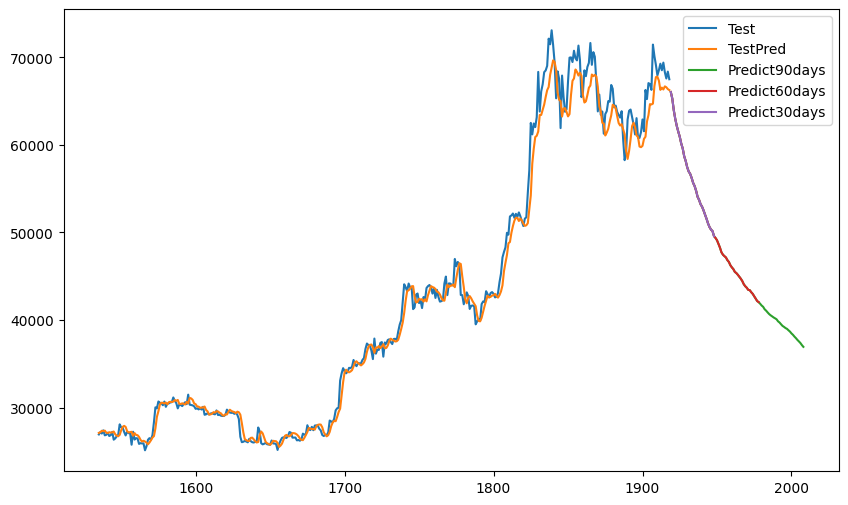
\includegraphics[width=1\linewidth]{image/BTC_RNN_82_Adam.png}
    \caption{BTC RNN 82 Adam.}
  \end{minipage}
\end{figure}
% /////////
\begin{figure}[H]
  \centering
  \begin{minipage}{0.48\linewidth}
    \centering
    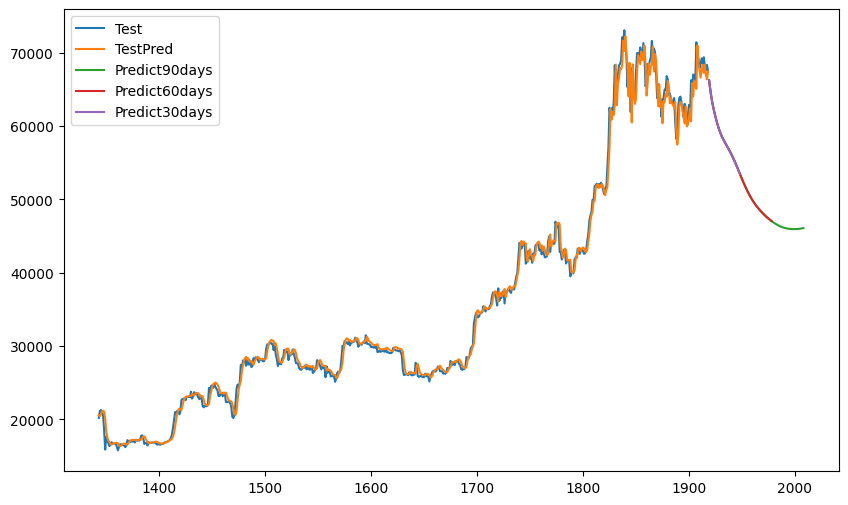
\includegraphics[width=1\linewidth]{image/BTC_LSTM_73_Adam.png}
    \caption{BTC LSTM 73 Adam.}
  \end{minipage}  
\hfill
  \begin{minipage}{0.48\linewidth}
    \centering
    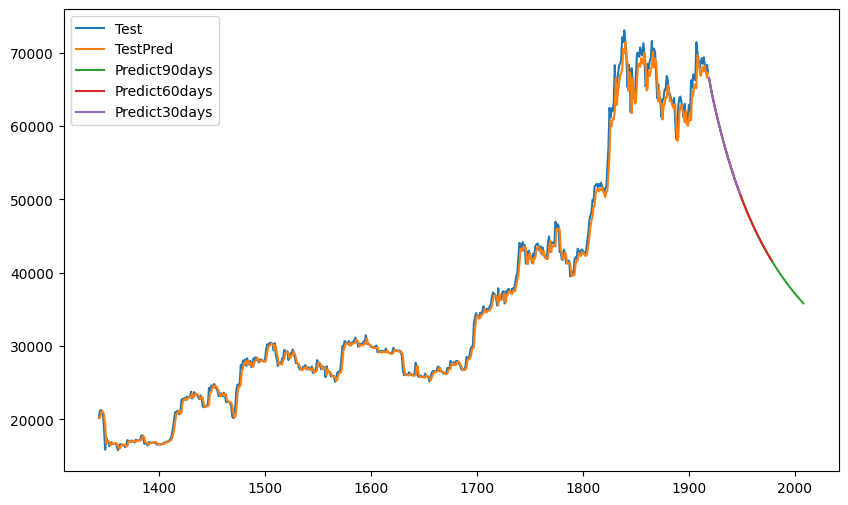
\includegraphics[width=1\linewidth]{image/BTC_GRU_73_Adam.png}
    \caption{BNB GRU 73 Adam.}
  \end{minipage}
\end{figure}

\begin{figure}[H]
  \centering
  \begin{minipage}{0.48\linewidth}
    \centering
    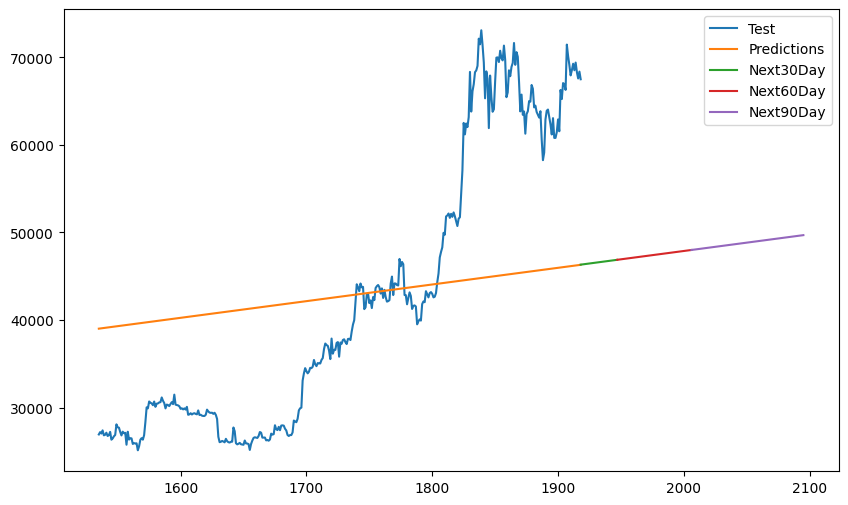
\includegraphics[width=1\linewidth]{image/BTC_LR_82.png}
    \caption{BTC LR 82.}
  \end{minipage}
\hfill
  \begin{minipage}{0.48\linewidth}
    \centering
    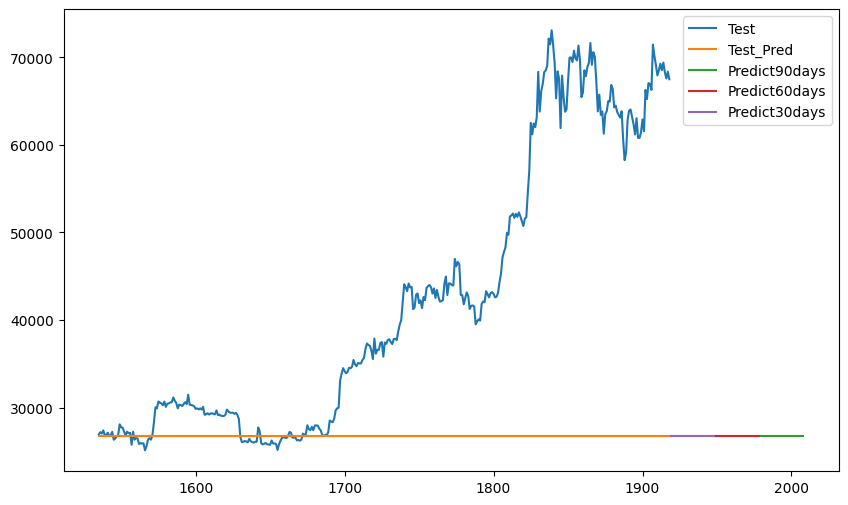
\includegraphics[width=1\linewidth]{image/BTC_ARIMA_82.png}
    \caption{BNB ARIMA 82.}
  \end{minipage}  
\end{figure}
% /////////////

\subsubsection{ETH DATASET}
\begin{table}[H]
    \centering
    \caption{Performance Metrics for Various Models and Optimizers}
    \definecolor{orange}{rgb}{1.0, 0.65, 0.0}
    \begin{tabular}{|c|c|c|c|c|c|}
        \hline
        \rowcolor{ao(english)}
        Model & Prop & Opti & RMSE & MAPE (\%) & MAE \\ \hline

        \multirow{6}{*}{D-Linear} & \multirow{3}{*}{7:3} & Adam & 946.06 & 34.47 & 707.83 \\ \cline{3-6}
        & & Adamax & 923.3 & 33.73 & 690.75 \\ \cline{3-6}
        & & \textbf{Ftrl} & \textbf{879.63} & \textbf{28.5} & \textbf{646.48} \\ \cline{2-6}
        & \multirow{3}{*}{8:2} & Adam & 943.71 & 30.85 & 725.52 \\ \cline{3-6}
        & & Adamax & 915.52 & 30.14 & 703.23 \\ \cline{3-6}
        & & \textbf{Ftrl} & \textbf{897.97} & \textbf{25.62} & \textbf{670.7} \\ \cline{2-6}
        & \multirow{3}{*}{9:1} & Adam & 790.05 & 22.3 & 638.2 \\ \cline{3-6}
        & & \textbf{Adamax} & \textbf{789} & \textbf{22.25} & \textbf{637.52} \\ \cline{3-6}
        & & Ftrl & 972.2 & 25.76 & 798.72 \\ \hline
        
        \multirow{9}{*}{RNN} & \multirow{3}{*}{7:3} & \textbf{Adam} & \textbf{77.19} & \textbf{2.52} & \textbf{52.24}
        \\ \cline{3-6}
        & & Adamax & 84.82 & 2.53 & 53.88 \\ \cline{3-6}
        & & Ftrl & 1511.17 & 61.31 & 1343.52 \\ \cline{2-6}
        & \multirow{3}{*}{8:2} & \textbf{Adam} & \textbf{85.98} & \textbf{2.1} & \textbf{53.76} \\ \cline{3-6}
        & & Adamax & 107.35 & 3.46 & 79.66 \\ \cline{3-6}
        & & Ftrl & 1363.38 & 46.33 & 1173.75 \\ \cline{2-6}
        & \multirow{3}{*}{9:1} & \textbf{Adam} & \textbf{141.95} & \textbf{3.86} & \textbf{110.66} \\ \cline{3-6}
        & & Adamax & 129.75 & 3.29 & 94.48 \\ \cline{3-6}
        & & Ftrl & 1749.7 & 55.46 & 1651.6 \\ \hline
        
        \multirow{9}{*}{LSTM} & \multirow{3}{*}{7:3} & \textbf{Adam} & \textbf{72.99} & \textbf{2.17} & \textbf{46.07} \\ \cline{3-6}
         &  & Adamax & 138.15 & 5.77 & 111.85 \\ \cline{3-6}
         &  & Ftrl & 923.97 & 26.87 & 664.26 \\ \cline{2-6}
         & \multirow{3}{*}{8:2} & \textbf{Adam} & \textbf{80.83} & \textbf{2.1} & \textbf{52.24} \\ \cline{3-6}
         &  & Adamax & 105.35 & 3.15 & 74.51 \\ \cline{3-6}
         &  & Ftrl & 1105.5 & 31.86 & 860.81 \\ \cline{2-6}
         & \multirow{3}{*}{9:1} & \textbf{Adam} & \textbf{108.95} & \textbf{2.72} & \textbf{79.57}
         \\ \cline{3-6}
         &  & Adamax & 133.53 & 3.23 & 95.85 \\ \cline{3-6}
         &  & Ftrl & 1490.23 & 45.44 & 1373.73 \\ \hline

         \multirow{9}{*}{GRU} & \multirow{3}{*}{7:3} & \textbf{Adam} & \textbf{80.32} & \textbf{2.26} & \textbf{50.69} \\ \cline{3-6}
            & & Adamax & 87.81 & 2.63 & 57.49 \\ \cline{3-6}
            & & Ftrl & 1709.07 & 72.91 & 1562.80 \\ \cline{2-6}
            & \multirow{3}{*}{8:2} & \textbf{Adam} & \textbf{79.93} & \textbf{2.29} & \textbf{54.68} \\ \cline{3-6}
            & & Adamax & 116.25 & 3.62 & 88.85 \\ \cline{3-6}
            & & Ftrl & 1902.57 & 73.98 & 1771.62 \\ \cline{2-6}
            & \multirow{3}{*}{9:1} & Adam & 116.68 & 2.81 & 83.57 \\ \cline{3-6}
            & & \textbf{Adamax} & \textbf{113.86} & \textbf{2.70} & \textbf{79.58} \\ \cline{3-6}
            & & Ftrl & 2342.14 & 77.75 & 2269.79 \\ \hline
            
         
       \multirow{3}{*}{LR} & 7:3 &  & 250.68 & 86.55 & 231.04 \\ \cline{2-6}
         & 8:2 &  & 196.76 & 69.90 & 178.59 \\ \cline{2-6}
         & 9:1 &  & \textbf{131.97} & \textbf{32.99} & \textbf{124.80}
\\ \hline


        \multirow{3}{*}{ARIMA} & 7:3 &  & \textbf{884.49} & \textbf{24.82} & \textbf{617.90} \\ \cline{2-6}
         & 8:2 &  & 877.32 & 20.82 & 600.94 \\ \cline{2-6}
         & 9:1 &  & 1107.23 & 29.96 & 944.61 \\ \hline

         
    \end{tabular}
\end{table}

\textbf{Prediction next 30/60/90 days (the best models)}
\begin{figure}[H]
  \centering
  \begin{minipage}{0.48\linewidth}
    \centering
    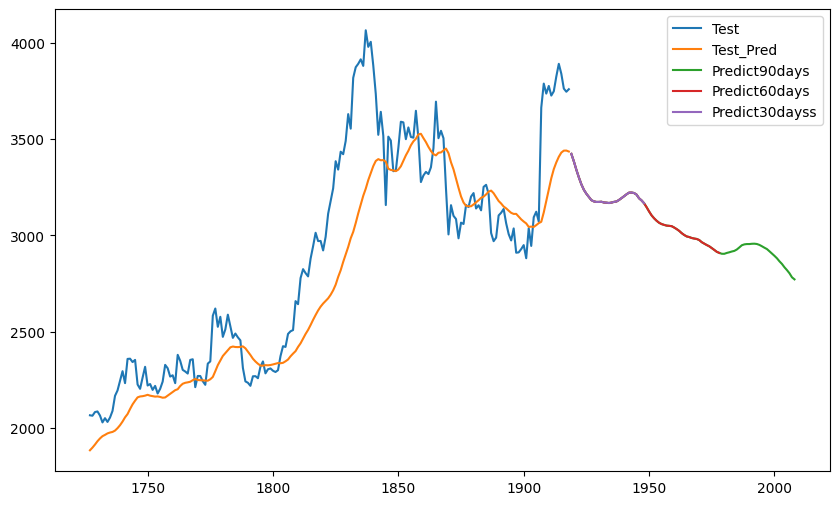
\includegraphics[width=1\linewidth]{image/ETH_DLinear_91_Adamax.png}
    \caption{ETH DLinear 91 Adamax.}
  \end{minipage}
\hfill
  \begin{minipage}{0.48\linewidth}
    \centering
    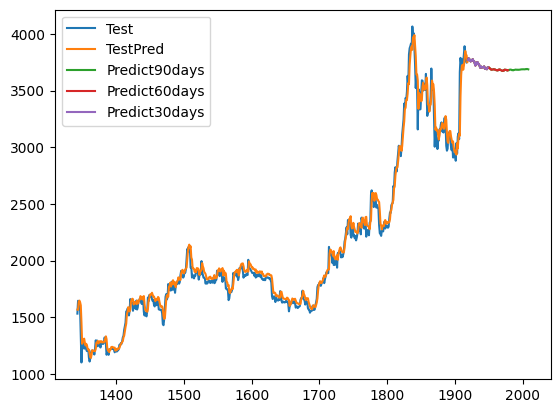
\includegraphics[width=1\linewidth]{image/ETH_RNN_73_Adam.png}
    \caption{ETH RNN 73 Adam.}
  \end{minipage}
\end{figure}

\begin{figure}[H]
  \centering
  \begin{minipage}{0.48\linewidth}
    \centering
    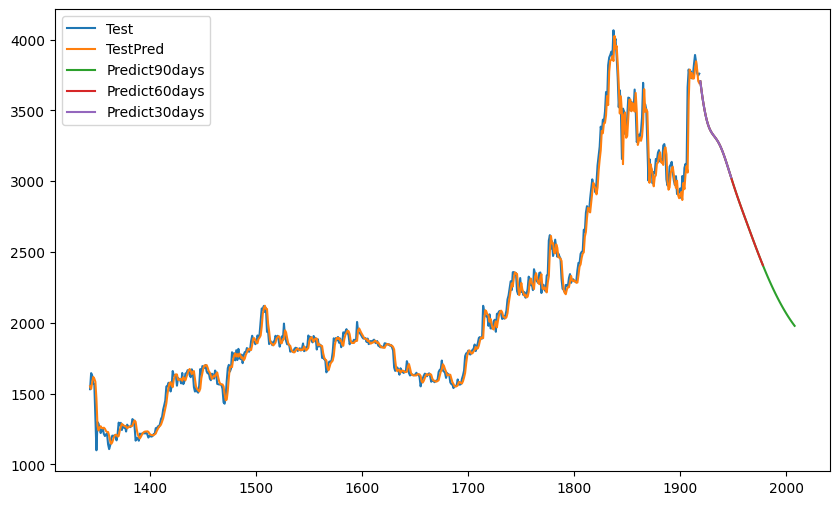
\includegraphics[width=1\linewidth]{image/ETH_LSTM_73_Adam.png}
    \caption{ETH LSTM 73 Adam.}
  \end{minipage}
\hfill
  \begin{minipage}{0.48\linewidth}
    \centering
    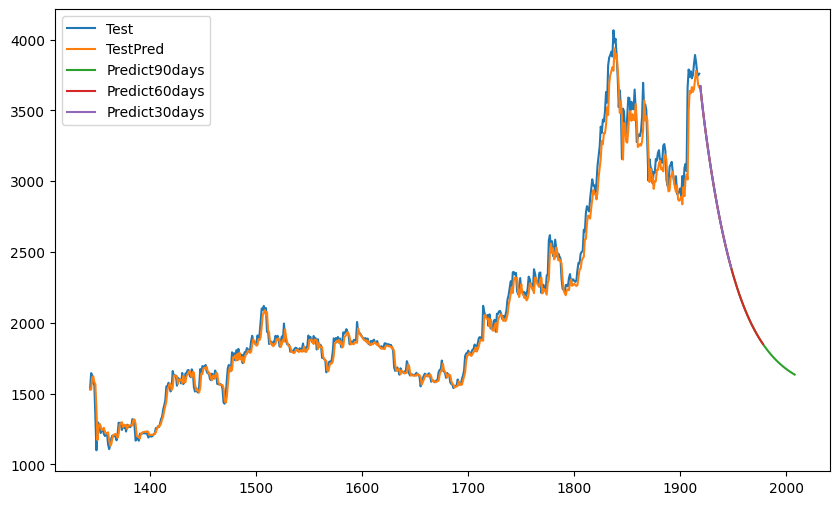
\includegraphics[width=1\linewidth]{image/ETH_GRU_73_Adam.png}
    \caption{ETH GRU 73 Adam.}
  \end{minipage}
\end{figure}

\begin{figure}[H]
  \centering
  \begin{minipage}{0.48\linewidth}
    \centering
    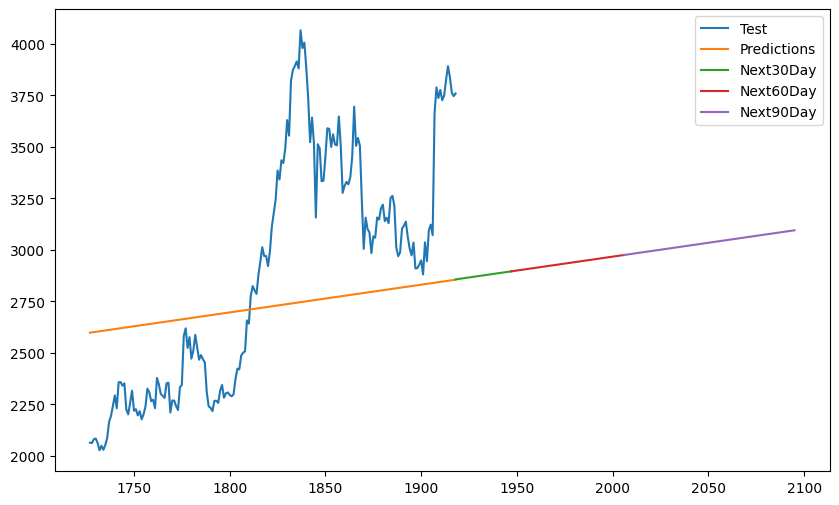
\includegraphics[width=1\linewidth]{image/ETH_LR_91.png}
    \caption{ETH LR 91.}
  \end{minipage}
    \hfill
  \begin{minipage}{0.48\linewidth}
    \centering
    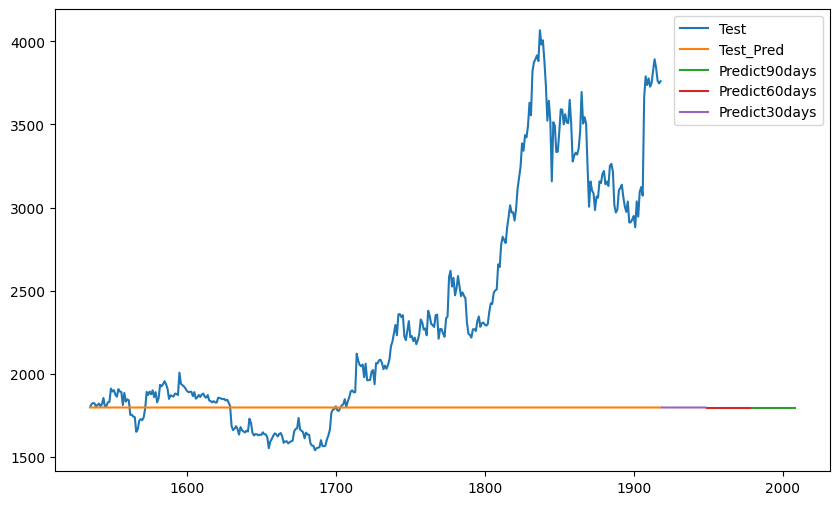
\includegraphics[width=1\linewidth]{image/ETH_ARIMA_82.png}
    \caption{BNB ARIMA 82.}
  \end{minipage}
\end{figure}
% /////////////

\subsection{RESULTS VISUALIZATION}
Below is charts comparing the optimizers according to each model corresponding to the \textbf{MAPE} metric with all rates. The outcomes shown that, in a variety of circumstances, Adam Optimizer generally achieved the lowest values for RMSE, MAPE, and MAE. Adamax accomplished well for DLinear and GRU models in only 2 cases compared to Adam Optimizer. Ftrl Optimizer's performance virtually ranked in the last across almost all scenarios.
\subsubsection{BNB DATASET}


\begin{figure}[H]
    \centering
    \begin{minipage}{0.15\textwidth}
        \centering
        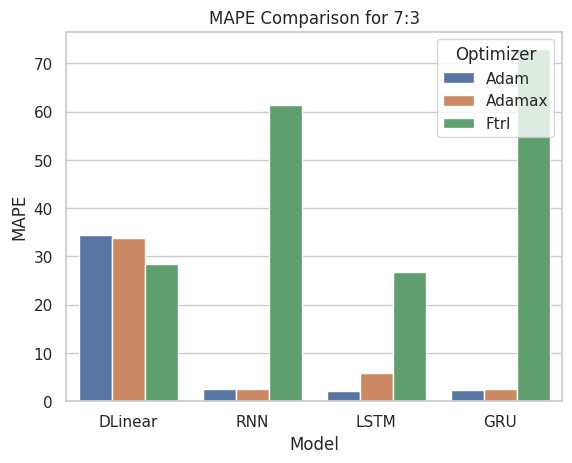
\includegraphics[width=1\textwidth]{image/MAPE_73_bnb.png}
        \caption{Comparision with 7:3}
        \label{fig:1}
    \end{minipage}%
    \hfill
    \begin{minipage}{0.15\textwidth}
        \centering
        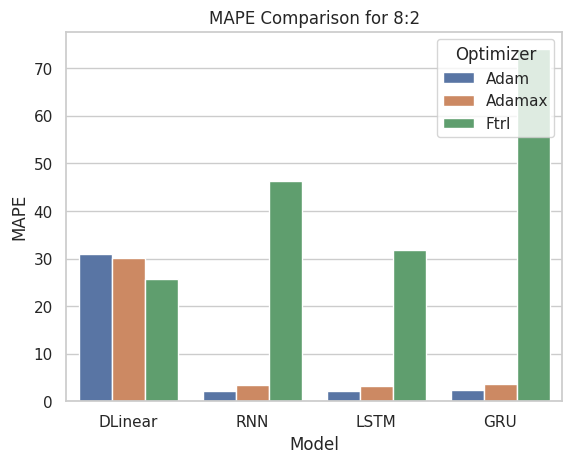
\includegraphics[width=1\textwidth]{image/MAPE_82_bnb.png}
        \caption{Comparision with 8:2}
        \label{fig:2}
    \end{minipage}%
    \hfill
    \begin{minipage}{0.15\textwidth}
        \centering
        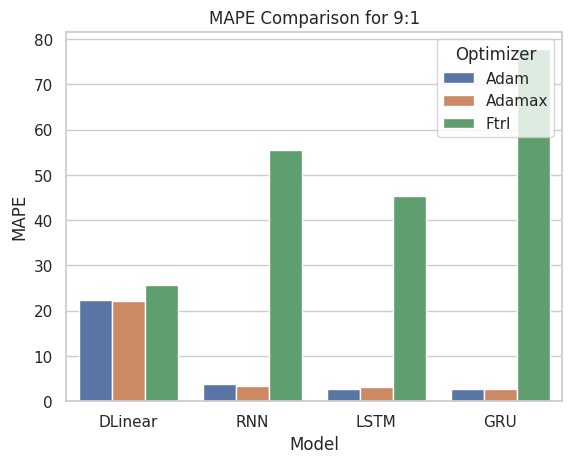
\includegraphics[width=1\textwidth]{image/MAPE_91_bnb.png}
        \caption{Comparision with 9:1}
        \label{fig:3}
    \end{minipage}
\end{figure}

% ////////////////////////////
\subsubsection{BTC DATASET}

\begin{figure}[H]
    \centering
    \begin{minipage}{0.15\textwidth}
    \centering
    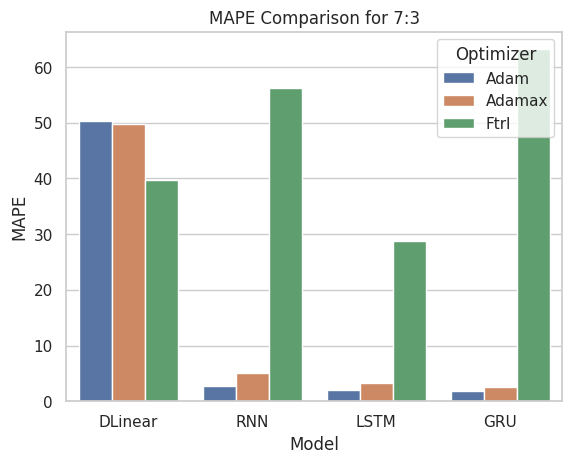
\includegraphics[width=1\textwidth]{image/MAPE_73_btc.png}
    \caption{Comparision with 7:3}
    \end{minipage}
    \hfill
    \begin{minipage}{0.15\textwidth}
    \centering
    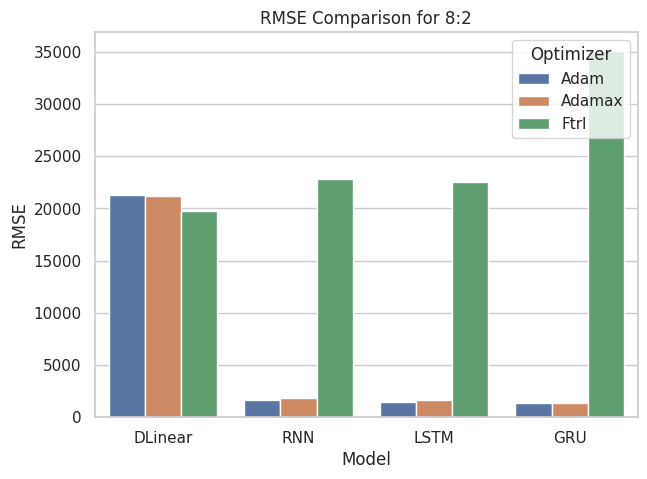
\includegraphics[width=1\textwidth]{image/MAPE_82_btc.png}
    \caption{Comparision with 8:2}
    \end{minipage}
    \hfill
    \begin{minipage}{0.15\textwidth}
    \centering
    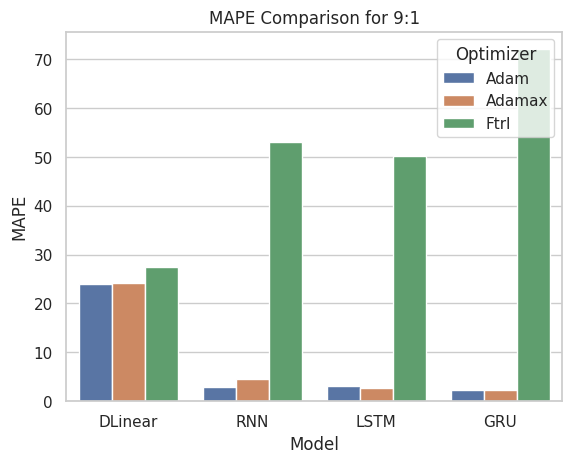
\includegraphics[width=1\textwidth]{image/MAPE_91_btc.png}
    \caption{Comparision with 9:1}
    \end{minipage}
\end{figure}
% ///////////////////
\subsubsection{ETH DATASET}
\begin{figure}[H]
    \centering
    \begin{minipage}{0.15\textwidth}
    \centering
    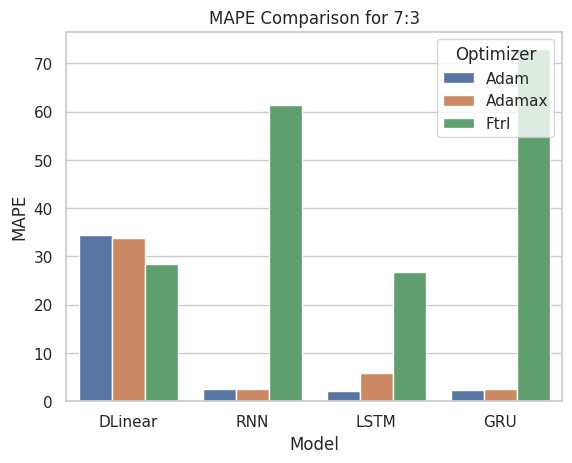
\includegraphics[width=1\textwidth]{image/MAPE_73_eth.png}
    \caption{Comparision with 7:3}
    \label{fig:1}
    \end{minipage}
    \hfill
    \begin{minipage}{0.15\textwidth}
    \centering
    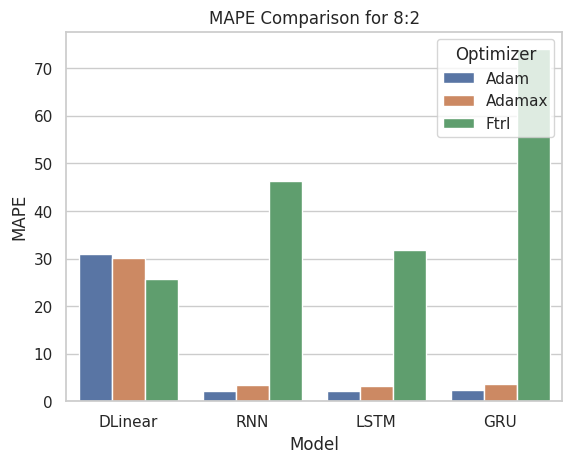
\includegraphics[width=1\textwidth]{image/MAPE_82_eth.png}
    \caption{Comparision with 8:2}
    \label{fig:2}
    \end{minipage}
    \hfill
    \begin{minipage}{0.15\textwidth}
    \centering
    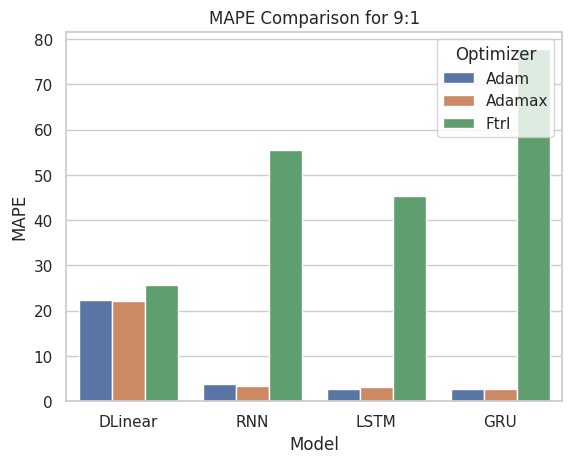
\includegraphics[width=1\textwidth]{image/MAPE_91_eth.png}
    \caption{Comparision 9:1}
    \label{fig:1}
    \end{minipage}
\end{figure}

\section{CONCLUSION}


\addcontentsline{toc}{section}{Acknowledgment}
\subsection{Summary}
\par In conclusion, our findings reveal that the choice of optimizer significantly influences the performance of predictive models in forecasting cryptocurrency prices. Among the optimization algorithms studied, Adam consistently outperformed Adamax and FTRL across all models and datasets, yielding the lowest RMSE, MAPE, and MAE values.
\\
Furthermore, our comprehensive evaluation underscores the critical role of optimization algorithms in forecasting cryptocurrency prices. The Adam optimizer consistently demonstrated superior performance across various models and datasets, highlighting its effectiveness in optimizing loss functions for predictive tasks. These insights not only contribute to the advancement of financial forecasting methodologies but also offer practical guidance for selecting appropriate optimizers in future research and applications within the domain of cryptocurrency market analysis.
\subsection{Future considerations}
\textbf {Automated Hyperparameter Tuning:}
Implement automated HPO methods to methodically search the hyperparameter space, such as Random Search, Grid Search, and Bayesian Optimization.
Utilize frameworks like Optuna, Hyperopt, or Ray Tune to streamline the optimization process.\\
\textbf {Ensemble Methods:}
Develop ensemble models that combine predictions from multiple algorithms to improve robustness and accuracy.
Experiment with techniques such as bagging, boosting, and stacking to leverage the strengths of various models.\\
\textbf {Using the other optimizers:}
Compare the performance of various optimizers (e.g., Adam, Adamax, RMSProp, Momentum, SGD, and Ftrl) and their hyperparameters to identify the best fit for the data..\\
\textbf {Learning-Rate Annealing Methods:}
The model can perform better on data that has not been seen by adjusting the learning rate during training, which helps the model better respond to the underlying patterns in the data. \cite{future_cons}.

% \end{thebibliography}
%%%%%%%%%%%%%%%
\section*{Acknowledgment}
Our supervisor, Assoc. Prof. Dr. Nguyen Dinh Thuan, has been instrumental in shaping the success of this endeavor with his expertise, insightful feedback, and mentorship. We would like to express our sincere gratitude to him for his invaluable guidance, continuous support, and unwavering commitment throughout the duration of this project.\\
We also extend our sincere appreciation to the teaching assistants, Ms Trinh Thi Thanh Truc and Ms Dang Vu Phuong Uyen, for their tireless efforts in providing hands-on support and practical guidance during the experimental and implementation phases of this work. Their dedication and willingness to share their knowledge have been truly instrumental in the completion of this project.\\

\bibliographystyle{plain}
\bibliography{mybibfile}
\EOD

\end{document}
